\part{全等与相似}
\section{全等三角形}
\subsection{基础定义}
\begin{definition}[全等关系]
    (1) 经过翻转、平移、旋转后,能够完全重合的两个三角形叫做全等三角形。
    
    (2) 若$\triangle ABC$与$\triangle DEF$全等,记作
    $$\triangle ABC \cong \triangle DEF.$$

    (3) 全等三角形的的三组对应边以及三组对应角全部相等,即
    $$\angle A = \angle D, \quad \angle B = \angle E, \quad \angle C = \angle F.$$
    $$AB = DE, \quad BC =EF, \quad AC=DF.$$
\end{definition}

\begin{figure}[h]
    \centering
    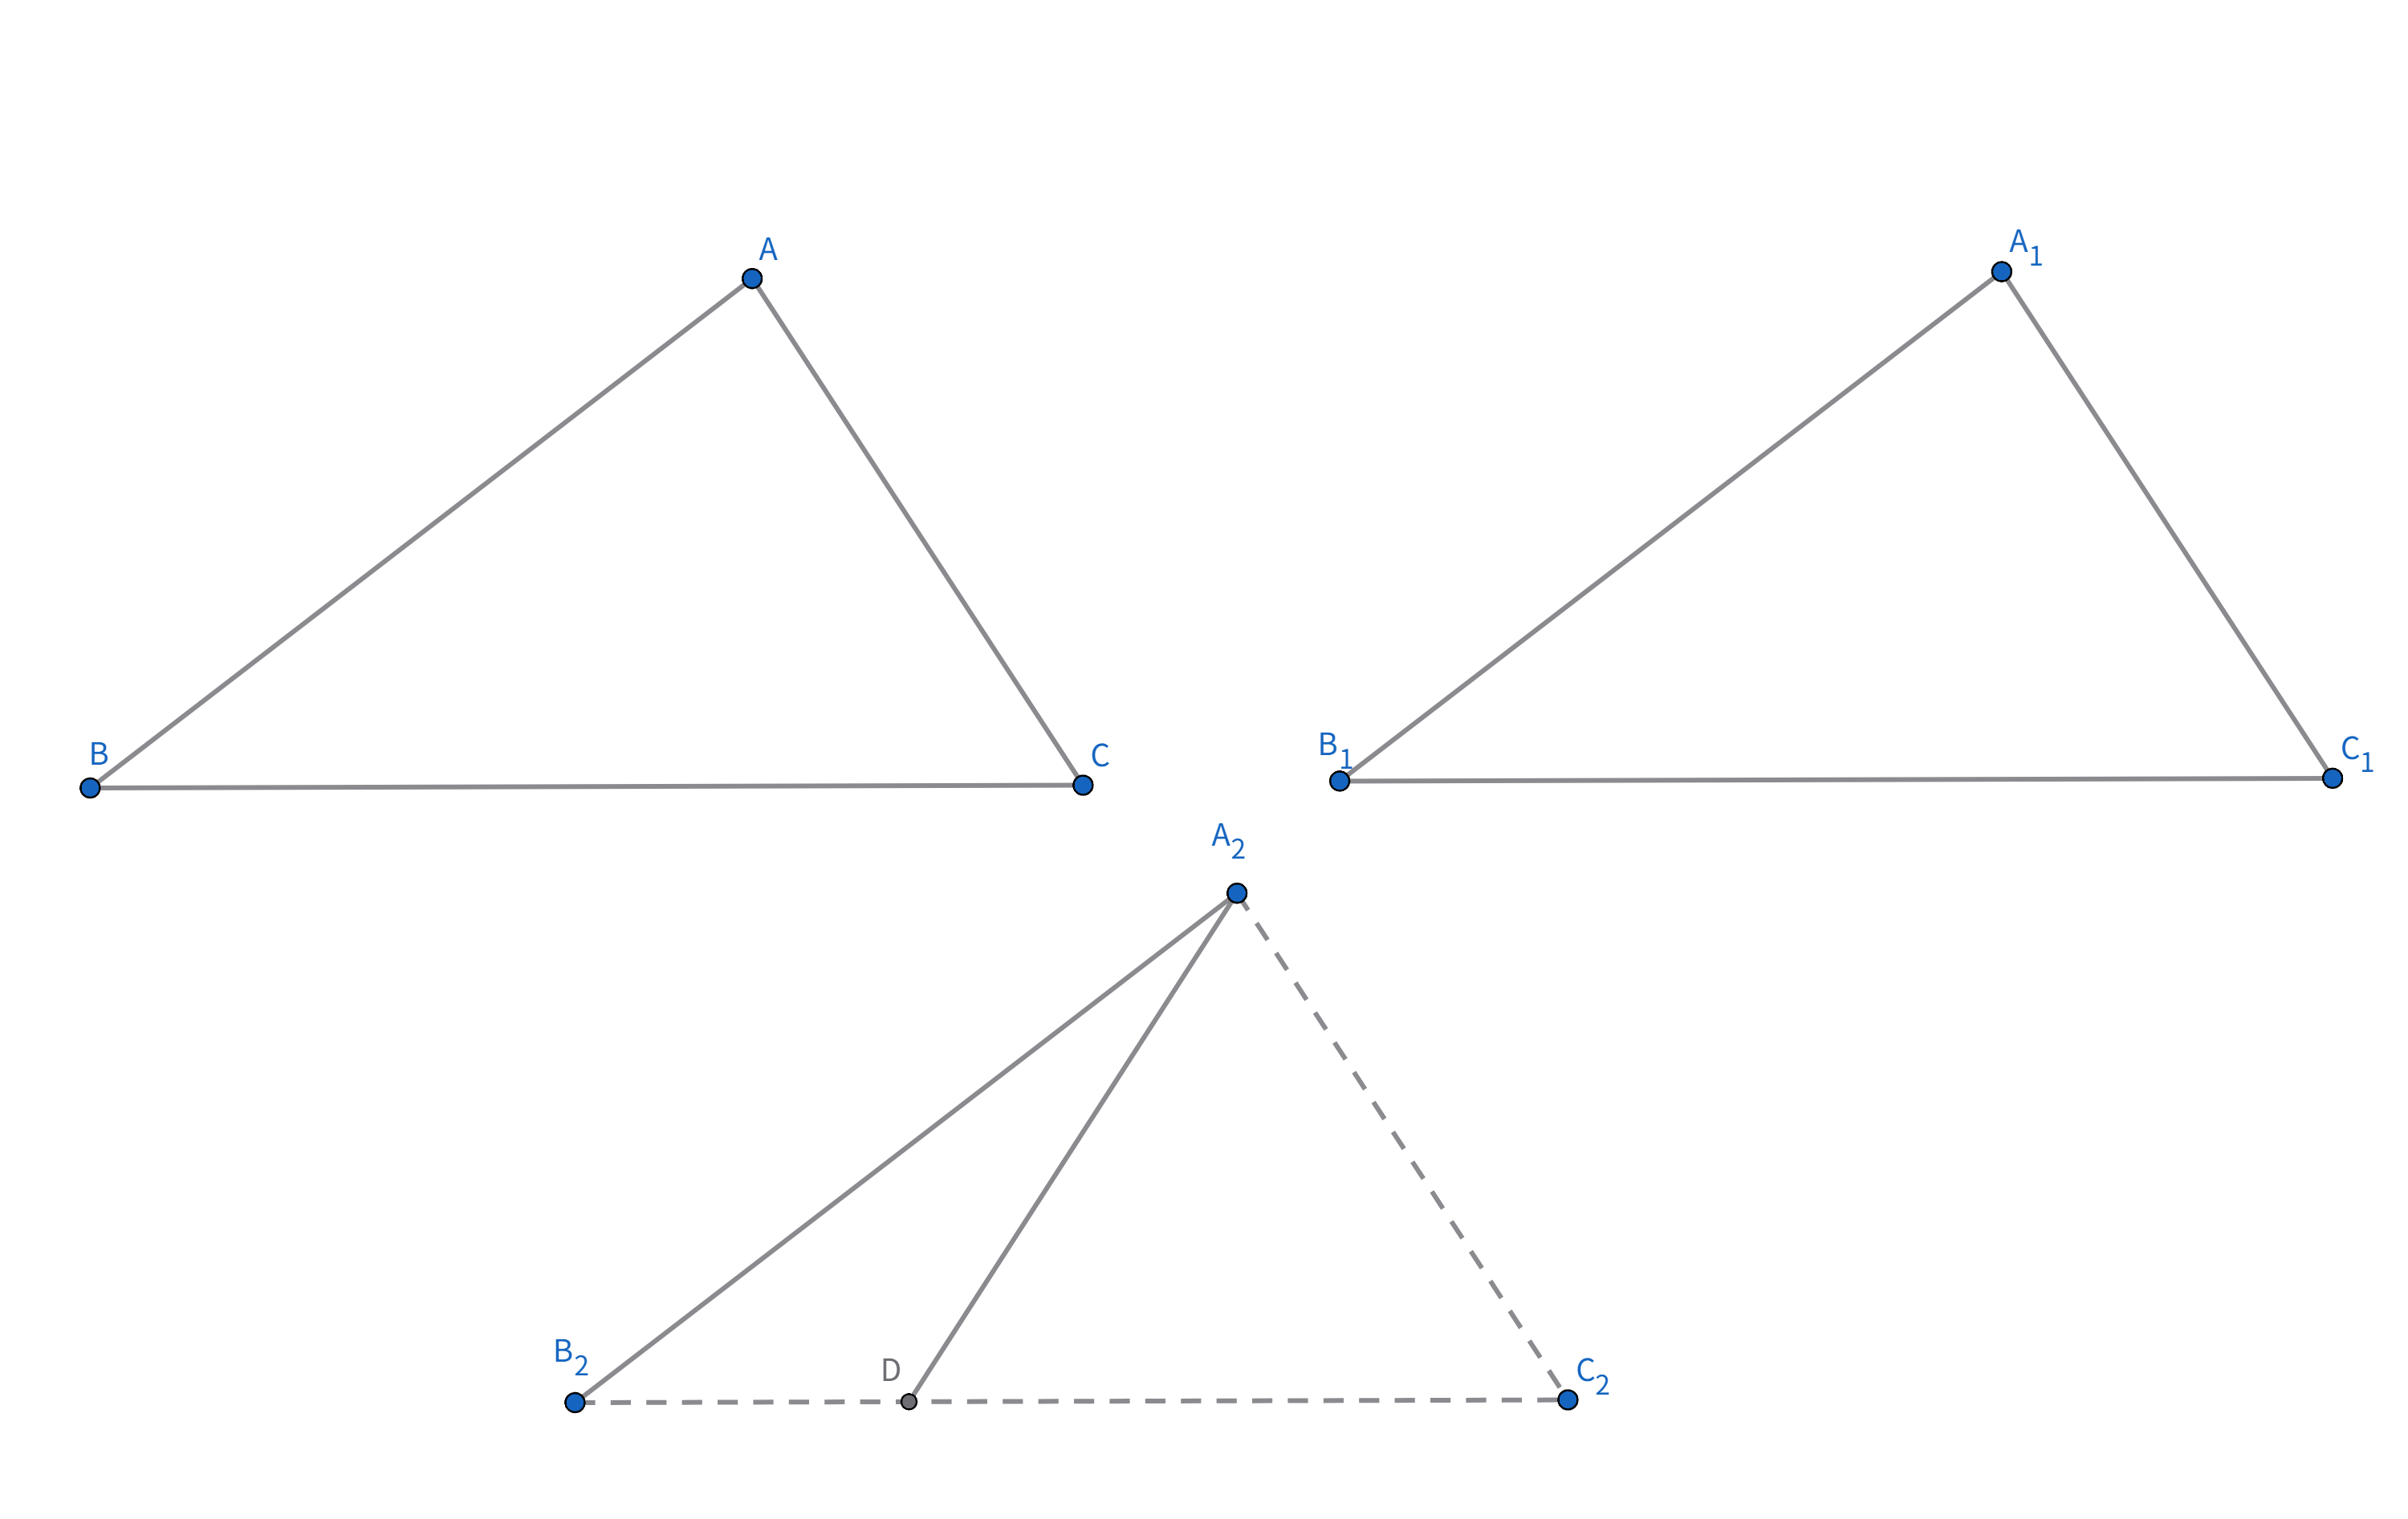
\includegraphics[width=\linewidth]{figures/全等三角形.png}
    \caption{边边角不能判定全等}
    % \label{fig:enter-label}
\end{figure}


\subsection{判定定理}
\begin{theorem}[全等三角形判定定理]
    若两三角形满足下列判别法中的其一,则一定全等。
    
    SSS (边边边): 三组边对应相等。

    SAS (边角边): 两边及其夹角对应相等。

    ASA (角边角): 两角及其夹边对应相等。

    AAS (角角边): 两角及其中一角的对边对应相等。
\end{theorem}

 
\section{平行线分线段成比例定理}
\begin{theorem}[平行线分线段成比例定理]
    假设有三条直线$l_1,l_2,l_3$互相平行,设另两条直线分别与$l_1,l_2,l_3$相交于$A,B,C$和$D,E,F$点。则
    $$\frac{AB}{BC} = \frac{DE}{EF},\quad 
    \frac{AB}{AC} = \frac{DE}{DF}, \quad 
    \frac{BC}{AC} = \frac{EF}{DF}$$
\end{theorem}
\begin{figure}[h]
    \centering
    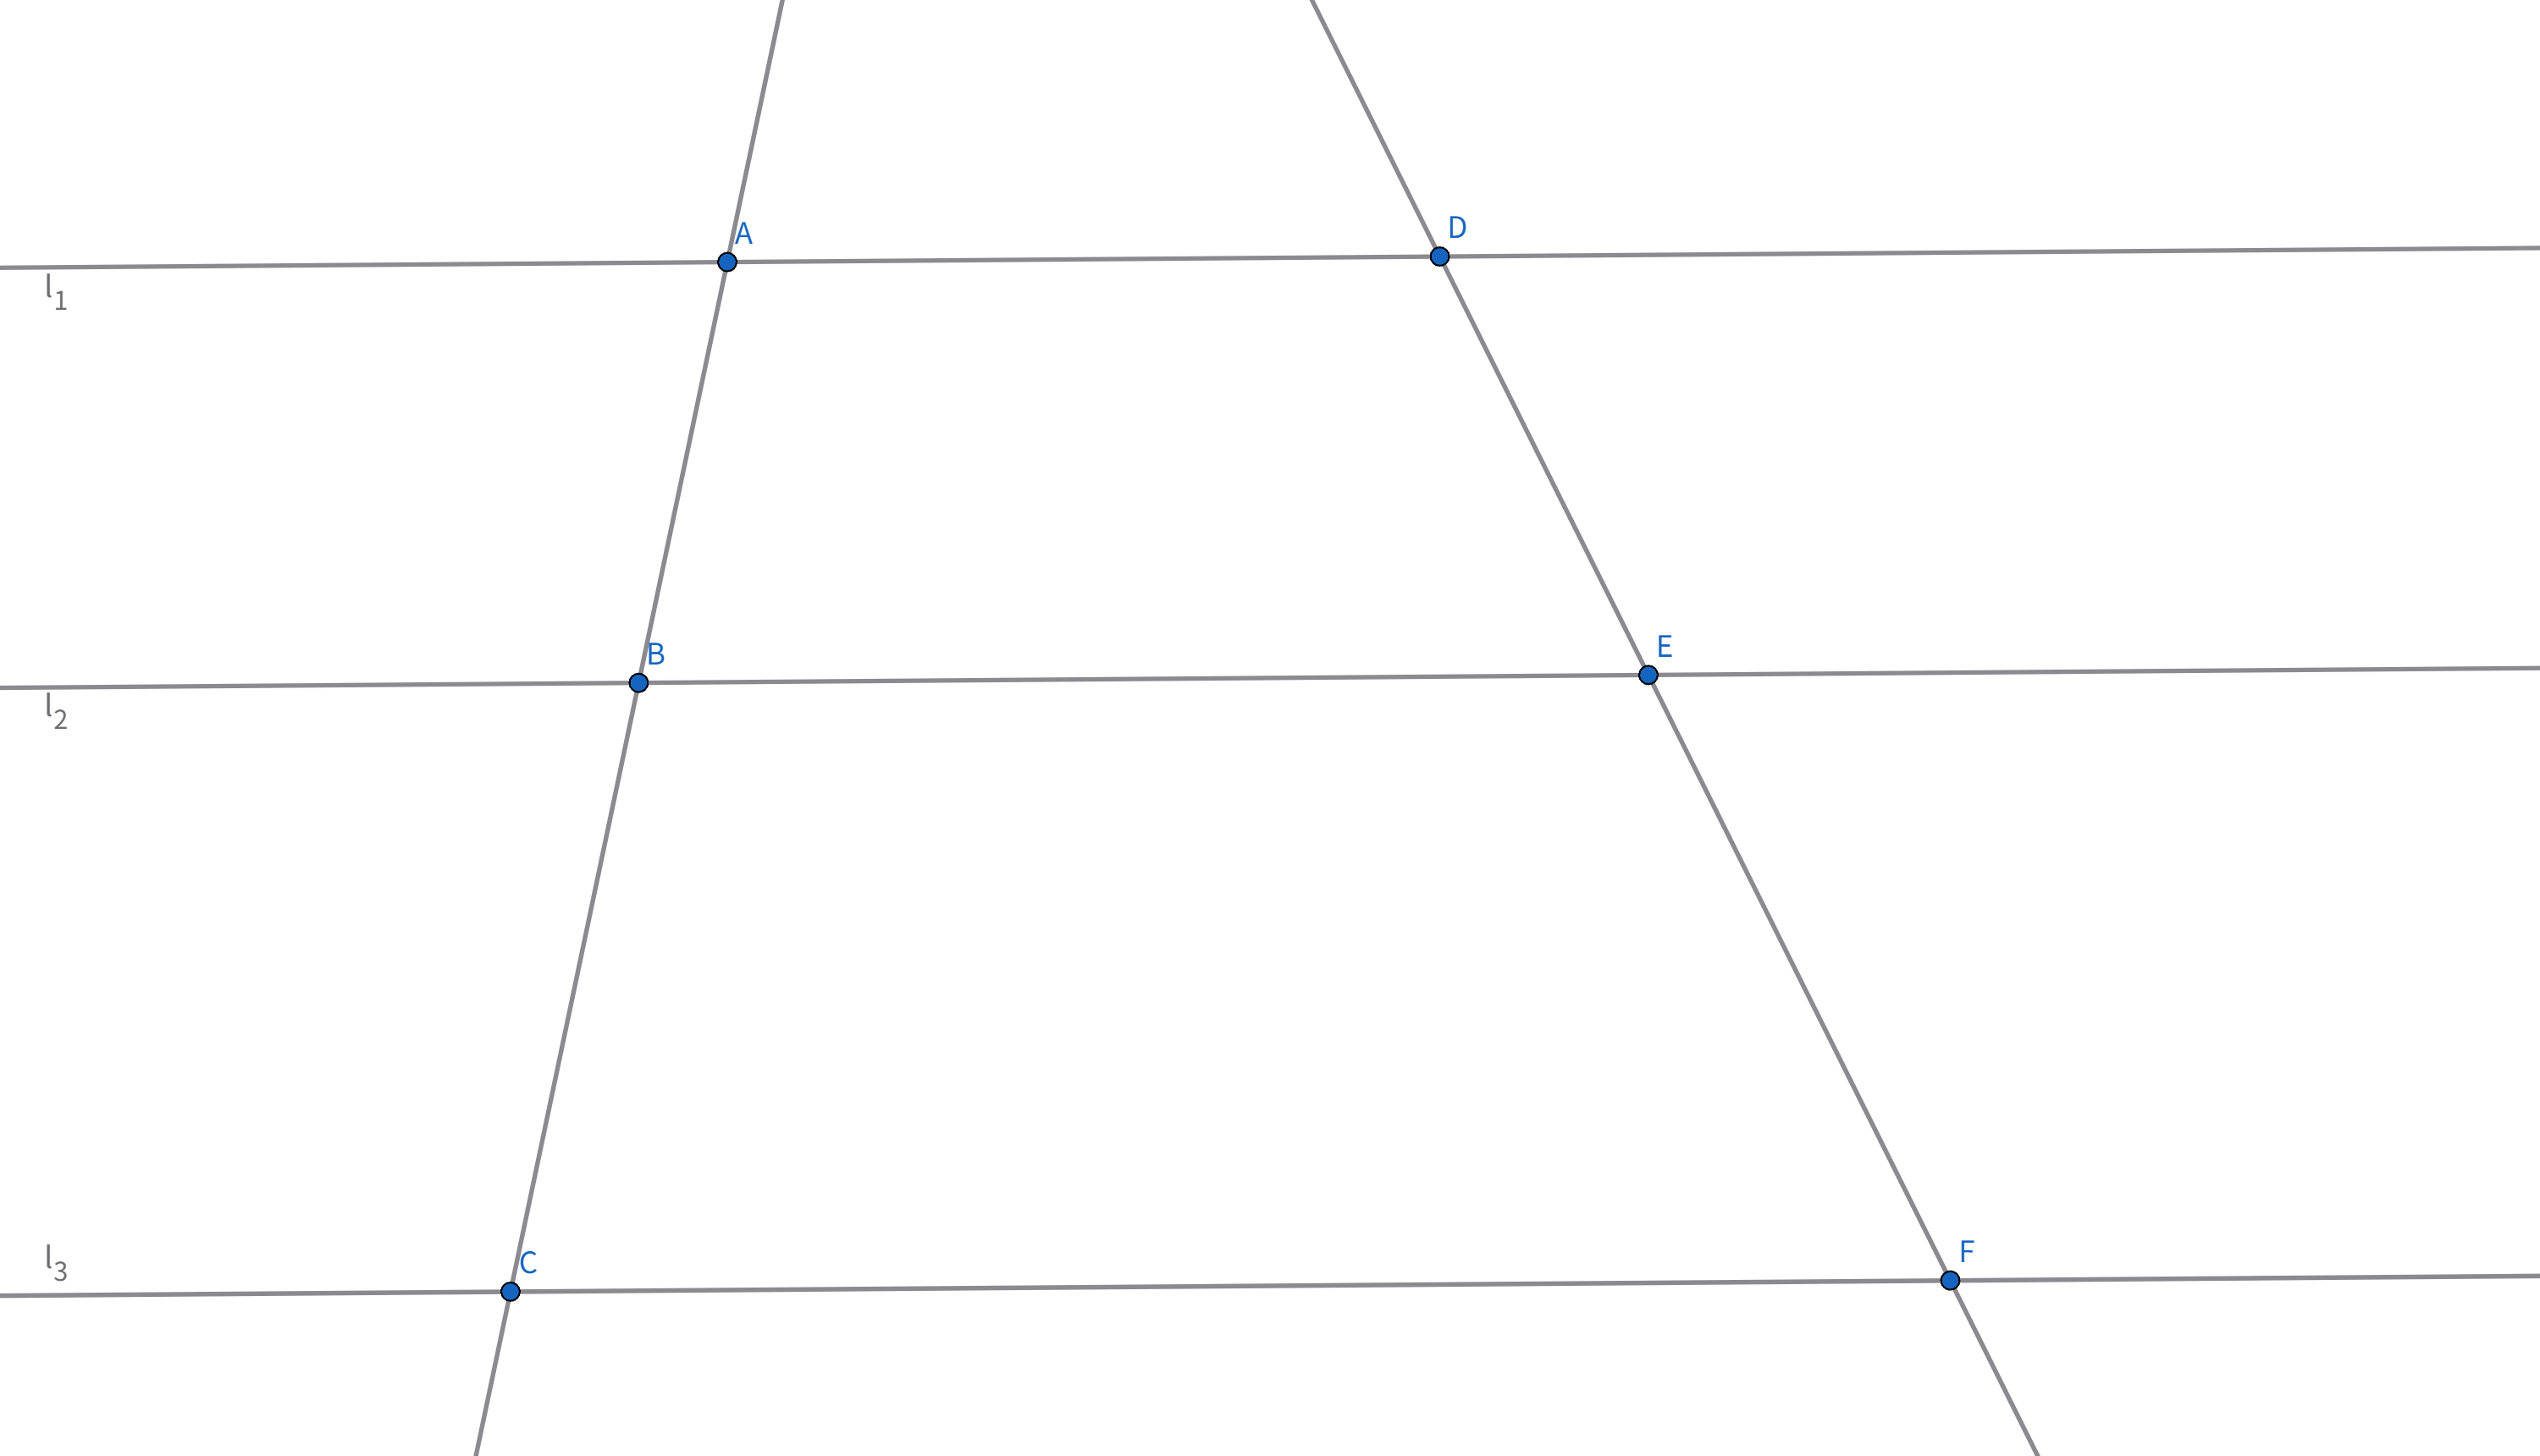
\includegraphics[width=0.8\linewidth]{figures/平行线分线段成比例.png}
    \caption{平行线分线段成比例}
    % \label{fig:enter-label}
\end{figure}

\begin{proposition}[平行相似]
    在$\triangle ABC$中,取AB、AC上的点DE平行于BC,则一定有$\triangle ABC \sim \triangle ADE$.
\end{proposition}

\begin{figure}[h]
    \centering
    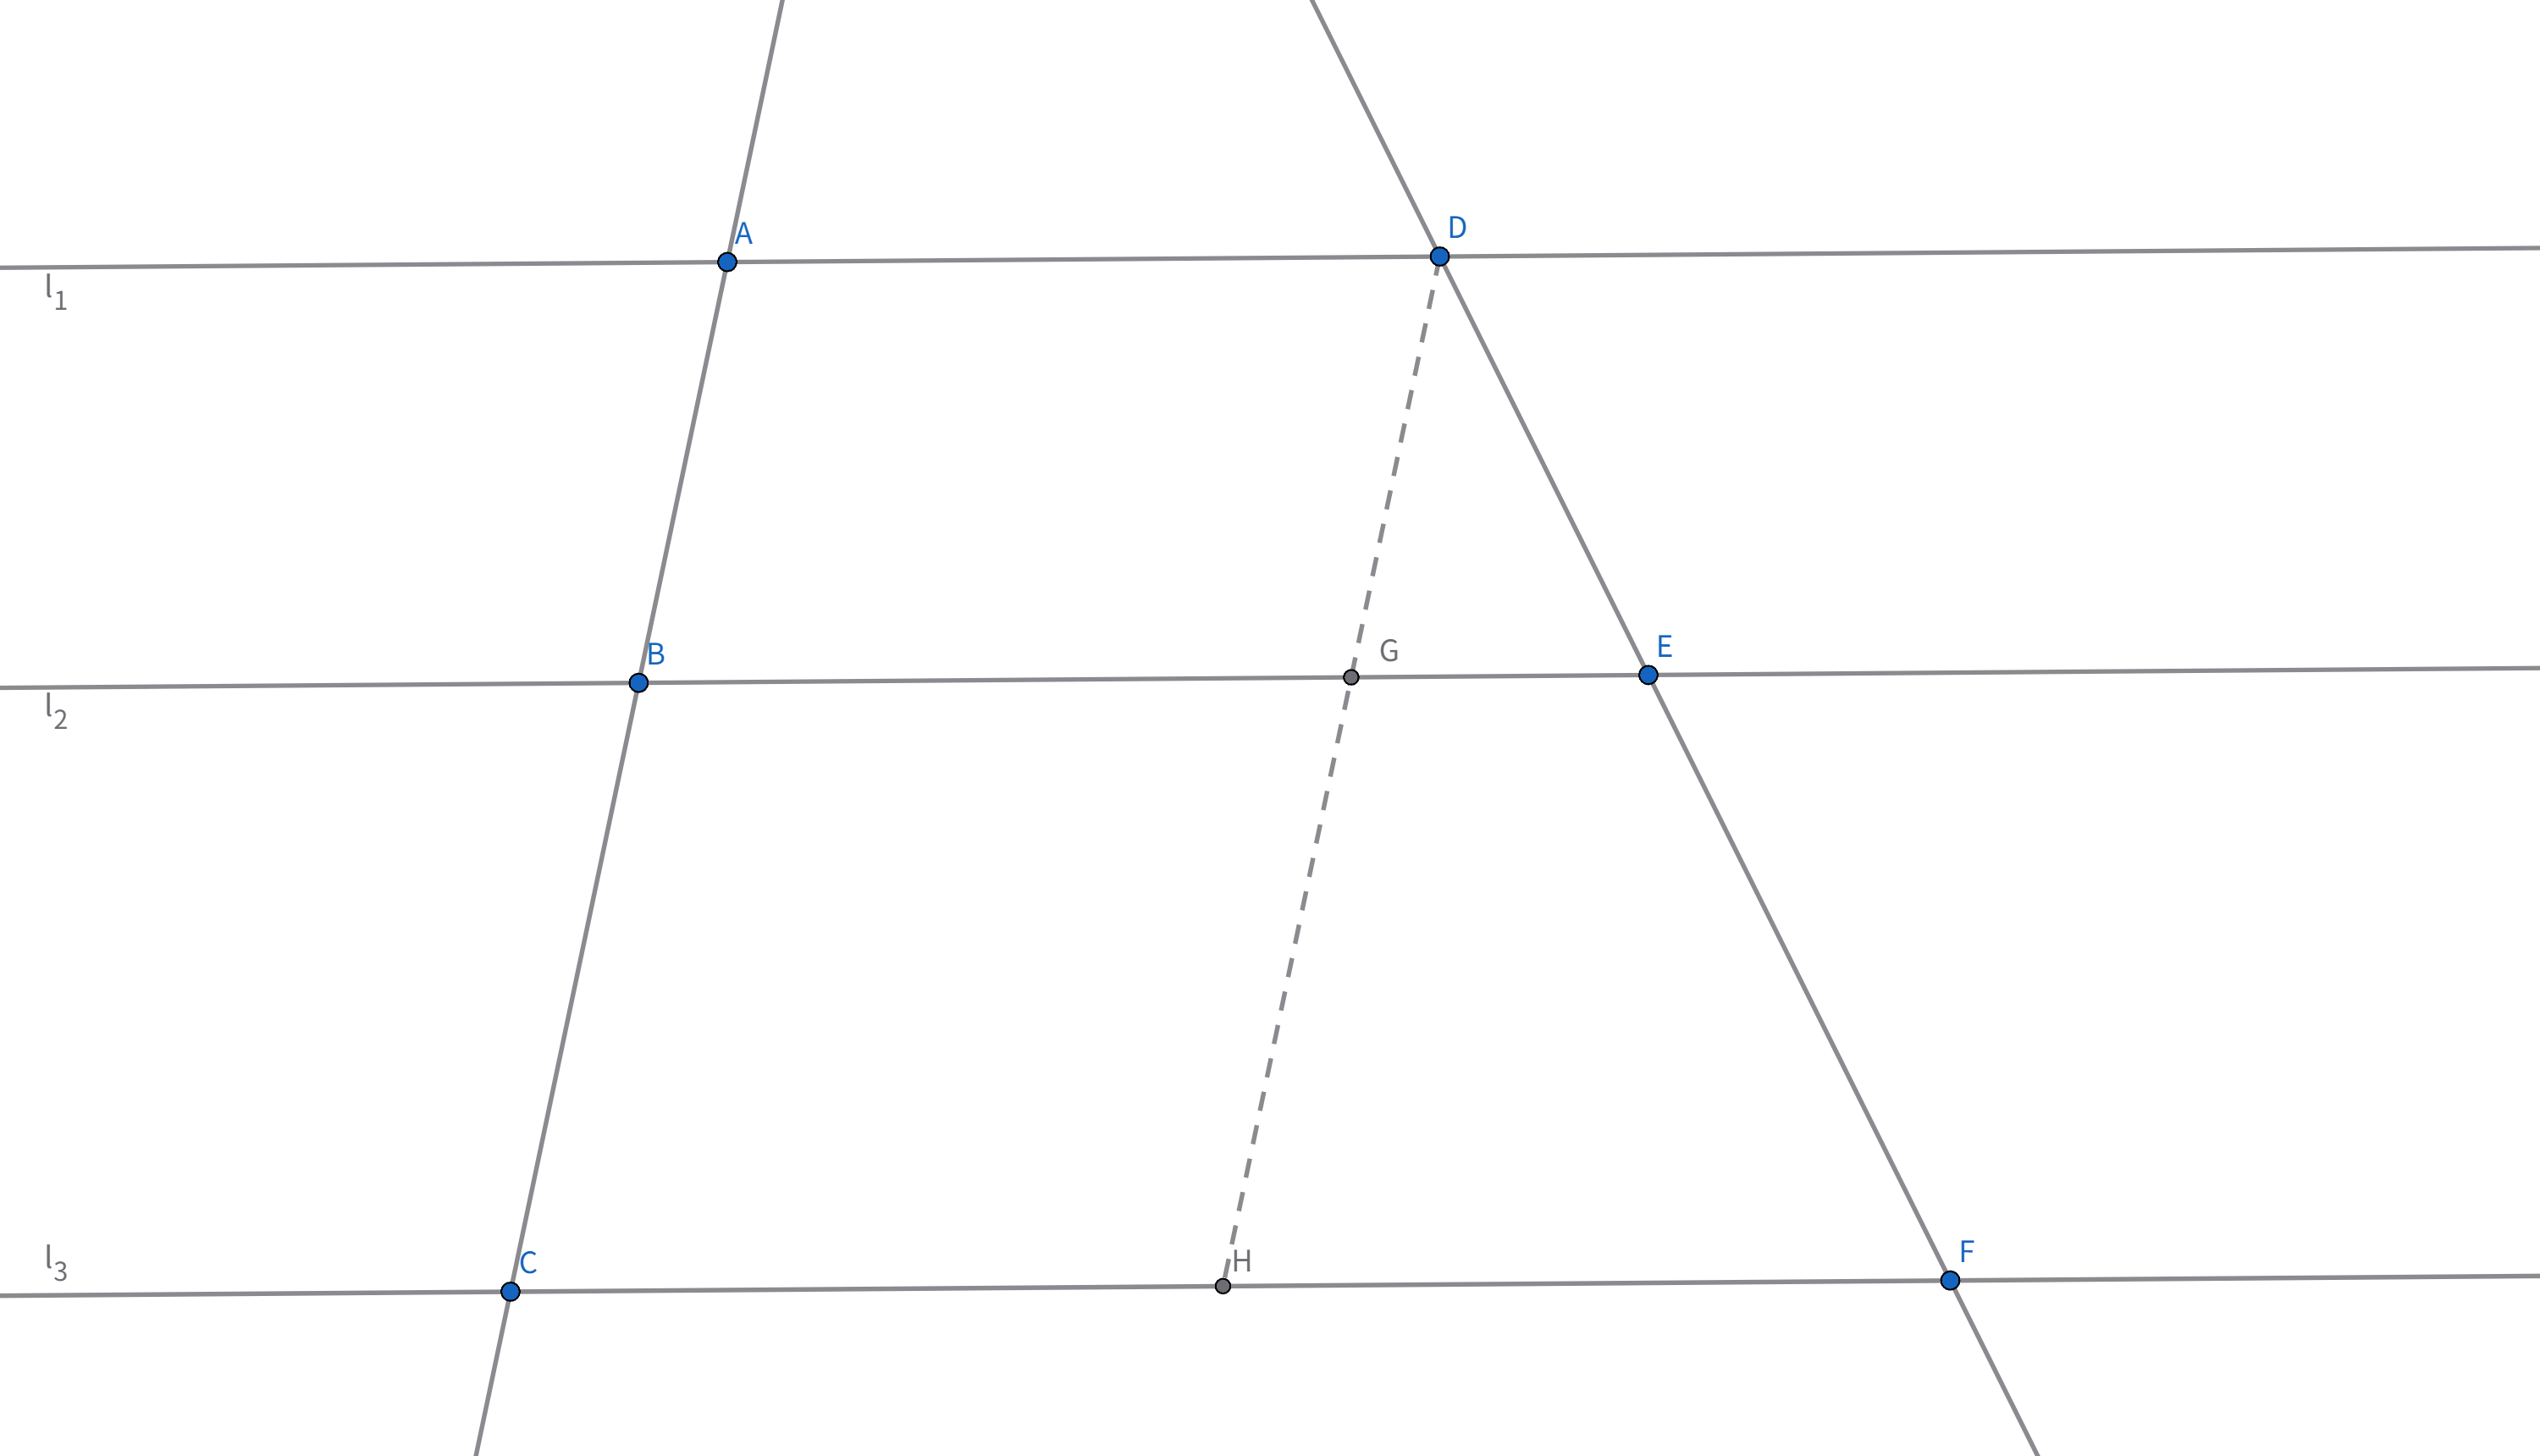
\includegraphics[width=0.8\linewidth]{figures/平行线分线段成比例 (1).png}
    \caption{平行相似}
    % \label{fig:enter-label}
\end{figure}


\section{相似三角形}
\subsection{基本概念}
\begin{definition}[相似关系]
(1) 对应角相等,对应边成比例的两个三角形叫做相似三角形。

(2) 若$\triangle ABC$与$\triangle DEF$相似,记作
    $$\triangle ABC \sim \triangle DEF.$$
(3) 相似三角形的三组对应角全部相等,即
    $$\angle A = \angle D, \quad \angle B = \angle E, \quad \angle C = \angle F.$$
(4) 相似三角形的三组对应边比例相等,即
    $$\frac{AB}{DE} = \frac{BC}{EF} = \frac{AC}{DF}=k.$$
    $k$称作是$\triangle ABC$与$\triangle DEF$的相似比。特别的,k=1时两三角形即为全等。
\end{definition}

\begin{figure}[h]
    \centering
    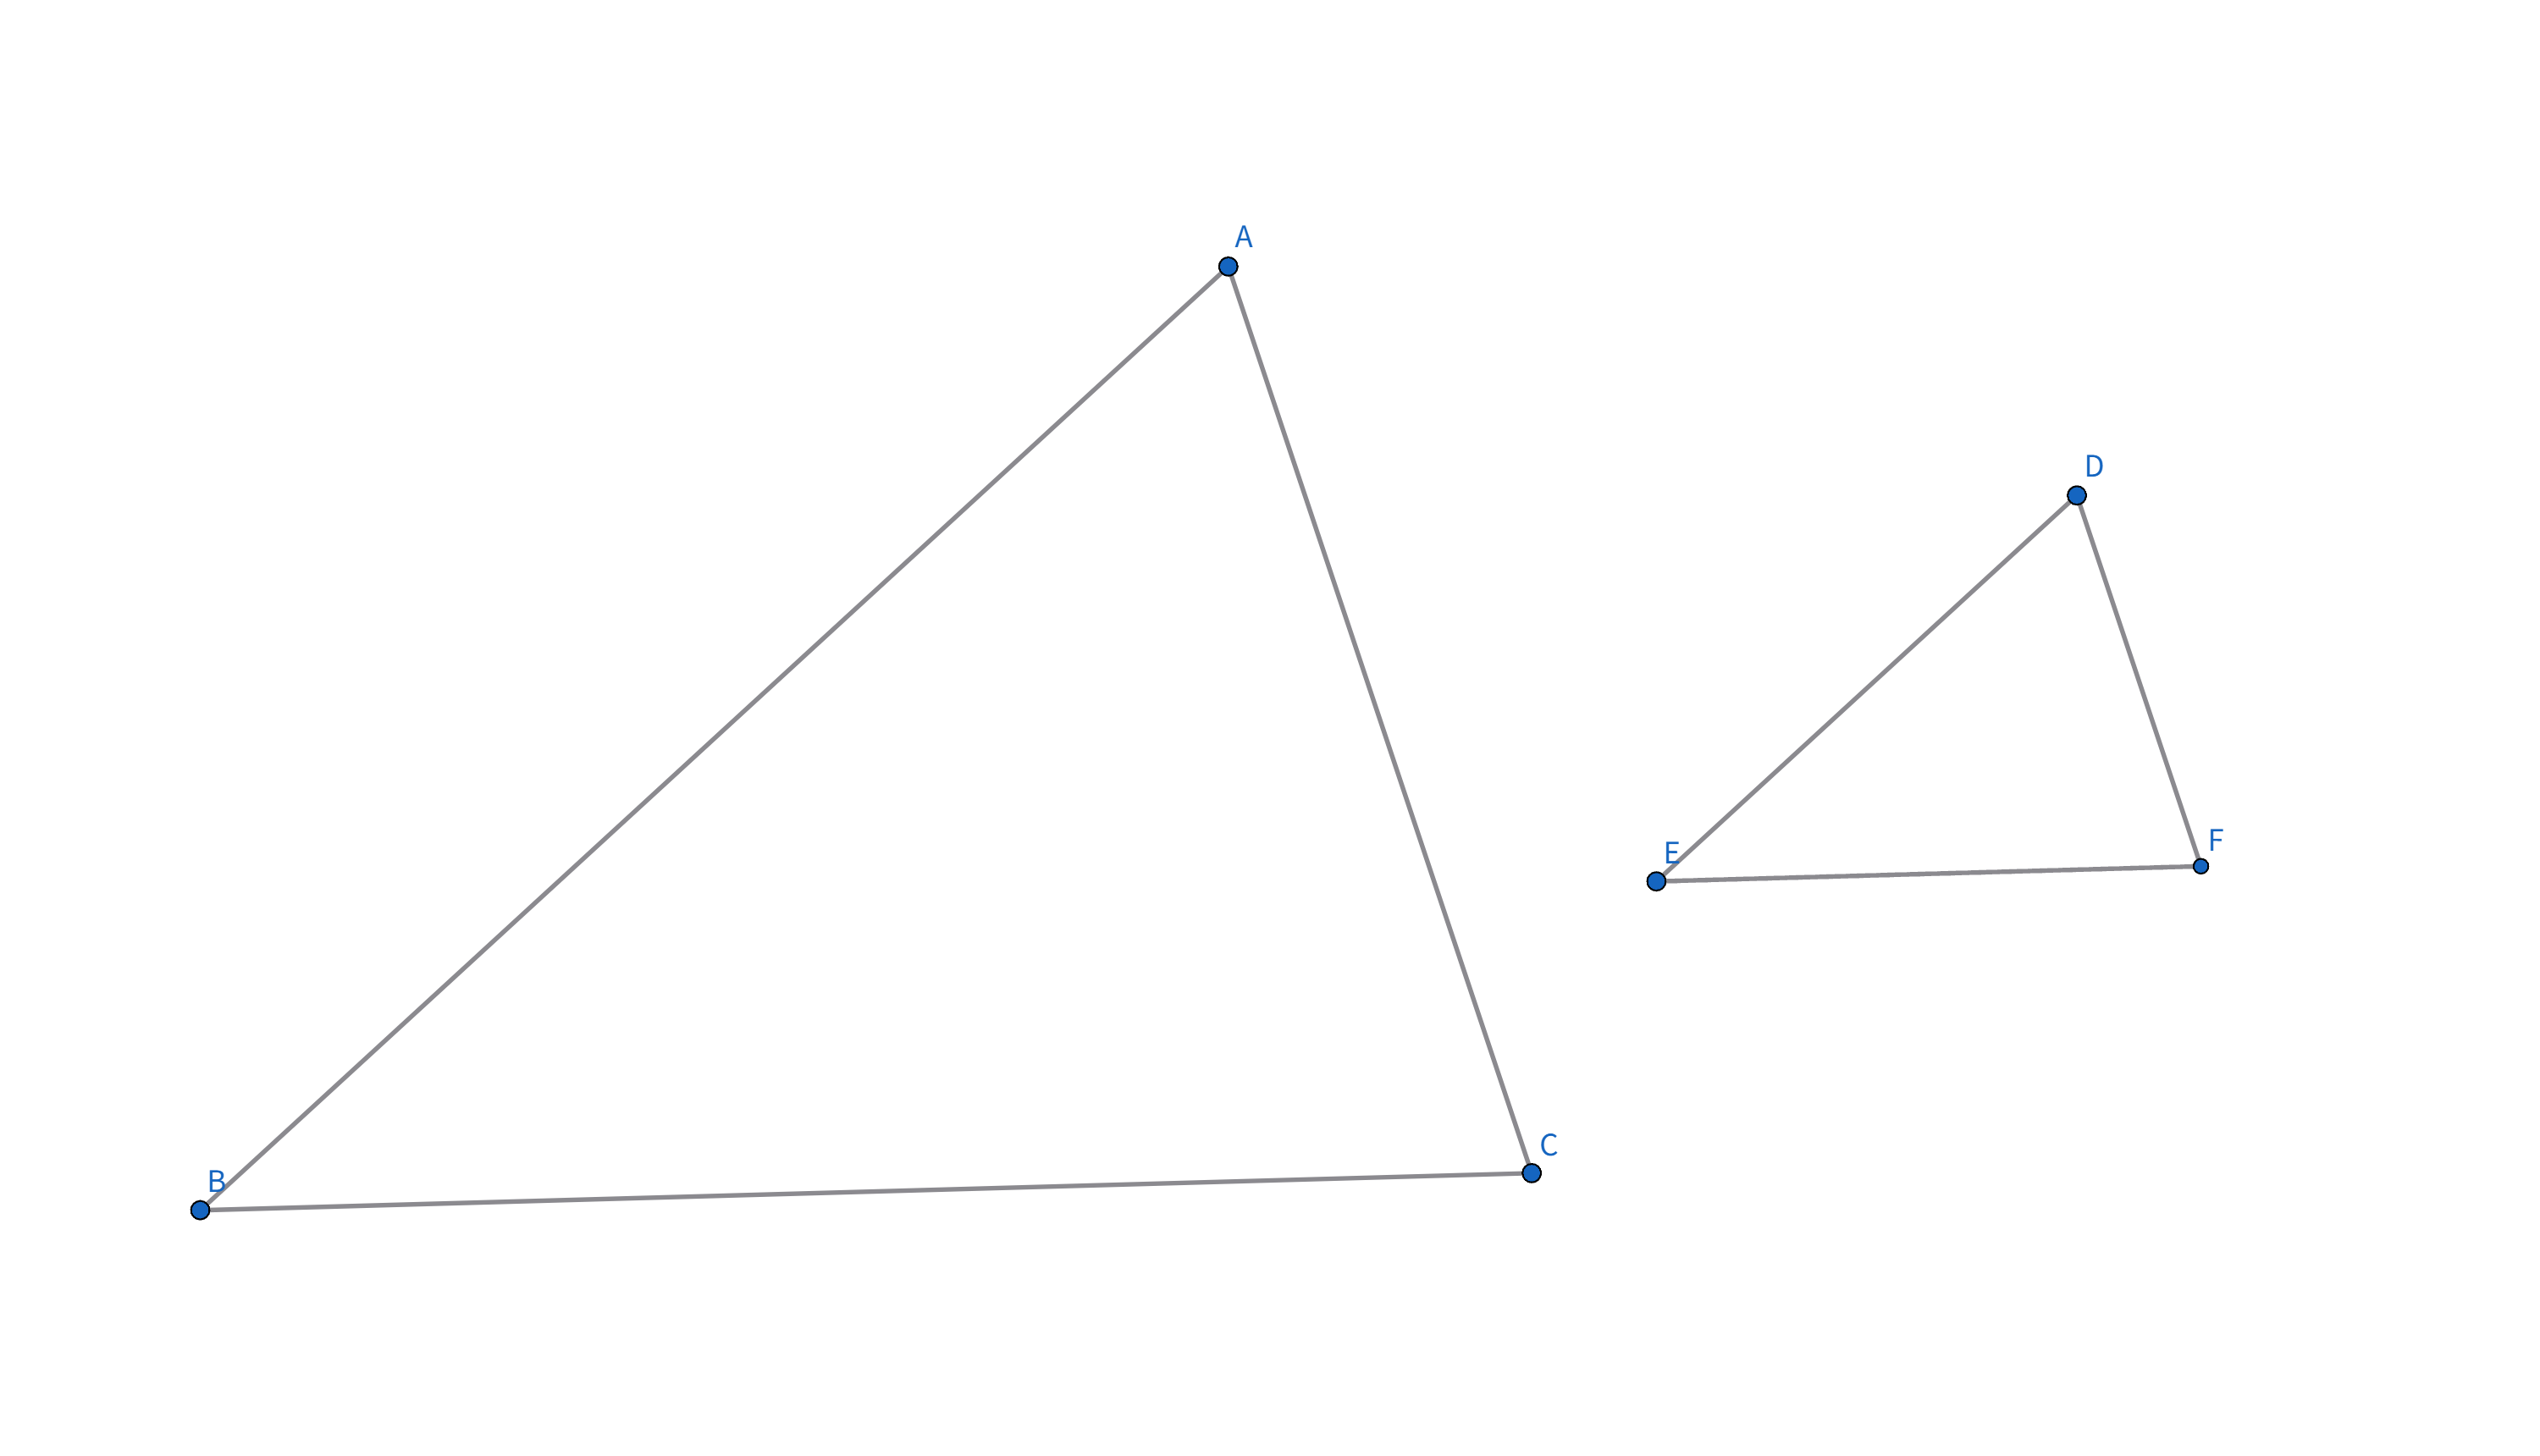
\includegraphics[width=0.8\linewidth]{figures/相似三角形.png}
    \caption{相似三角形}
    % \label{fig:enter-label}
\end{figure}
\begin{proposition}
    (5) 相似三角形的对应线段比也都等于相似比$k$,例如对应高线、角平分线、中线、中位线等。
    
    (6) 相似三角形的面积比为相似比的平方,即
    $$\frac{S_{\triangle ABC}}{S_{\triangle DEF}} = k^2.$$
    
    (6) 相似三角形同样具有传递性。
\end{proposition}

\subsection{判定定理}
\begin{theorem}
    若两三角形满足下列判别法中的其一,则一定相似。

    AA (角角) / AAA (角角角): 两角对应相等,则两三角形相似。
    
    SAS (边角边): 两边对应成比例且夹角相等,则两三角形相似。

    SSS (边边边): 三边对应成比例,则两三角形相似。
\end{theorem}
\begin{figure}[h]
    \centering
    \hfill % 添加一些水平间距
    \begin{minipage}[t]{0.3\textwidth}
        \centering
        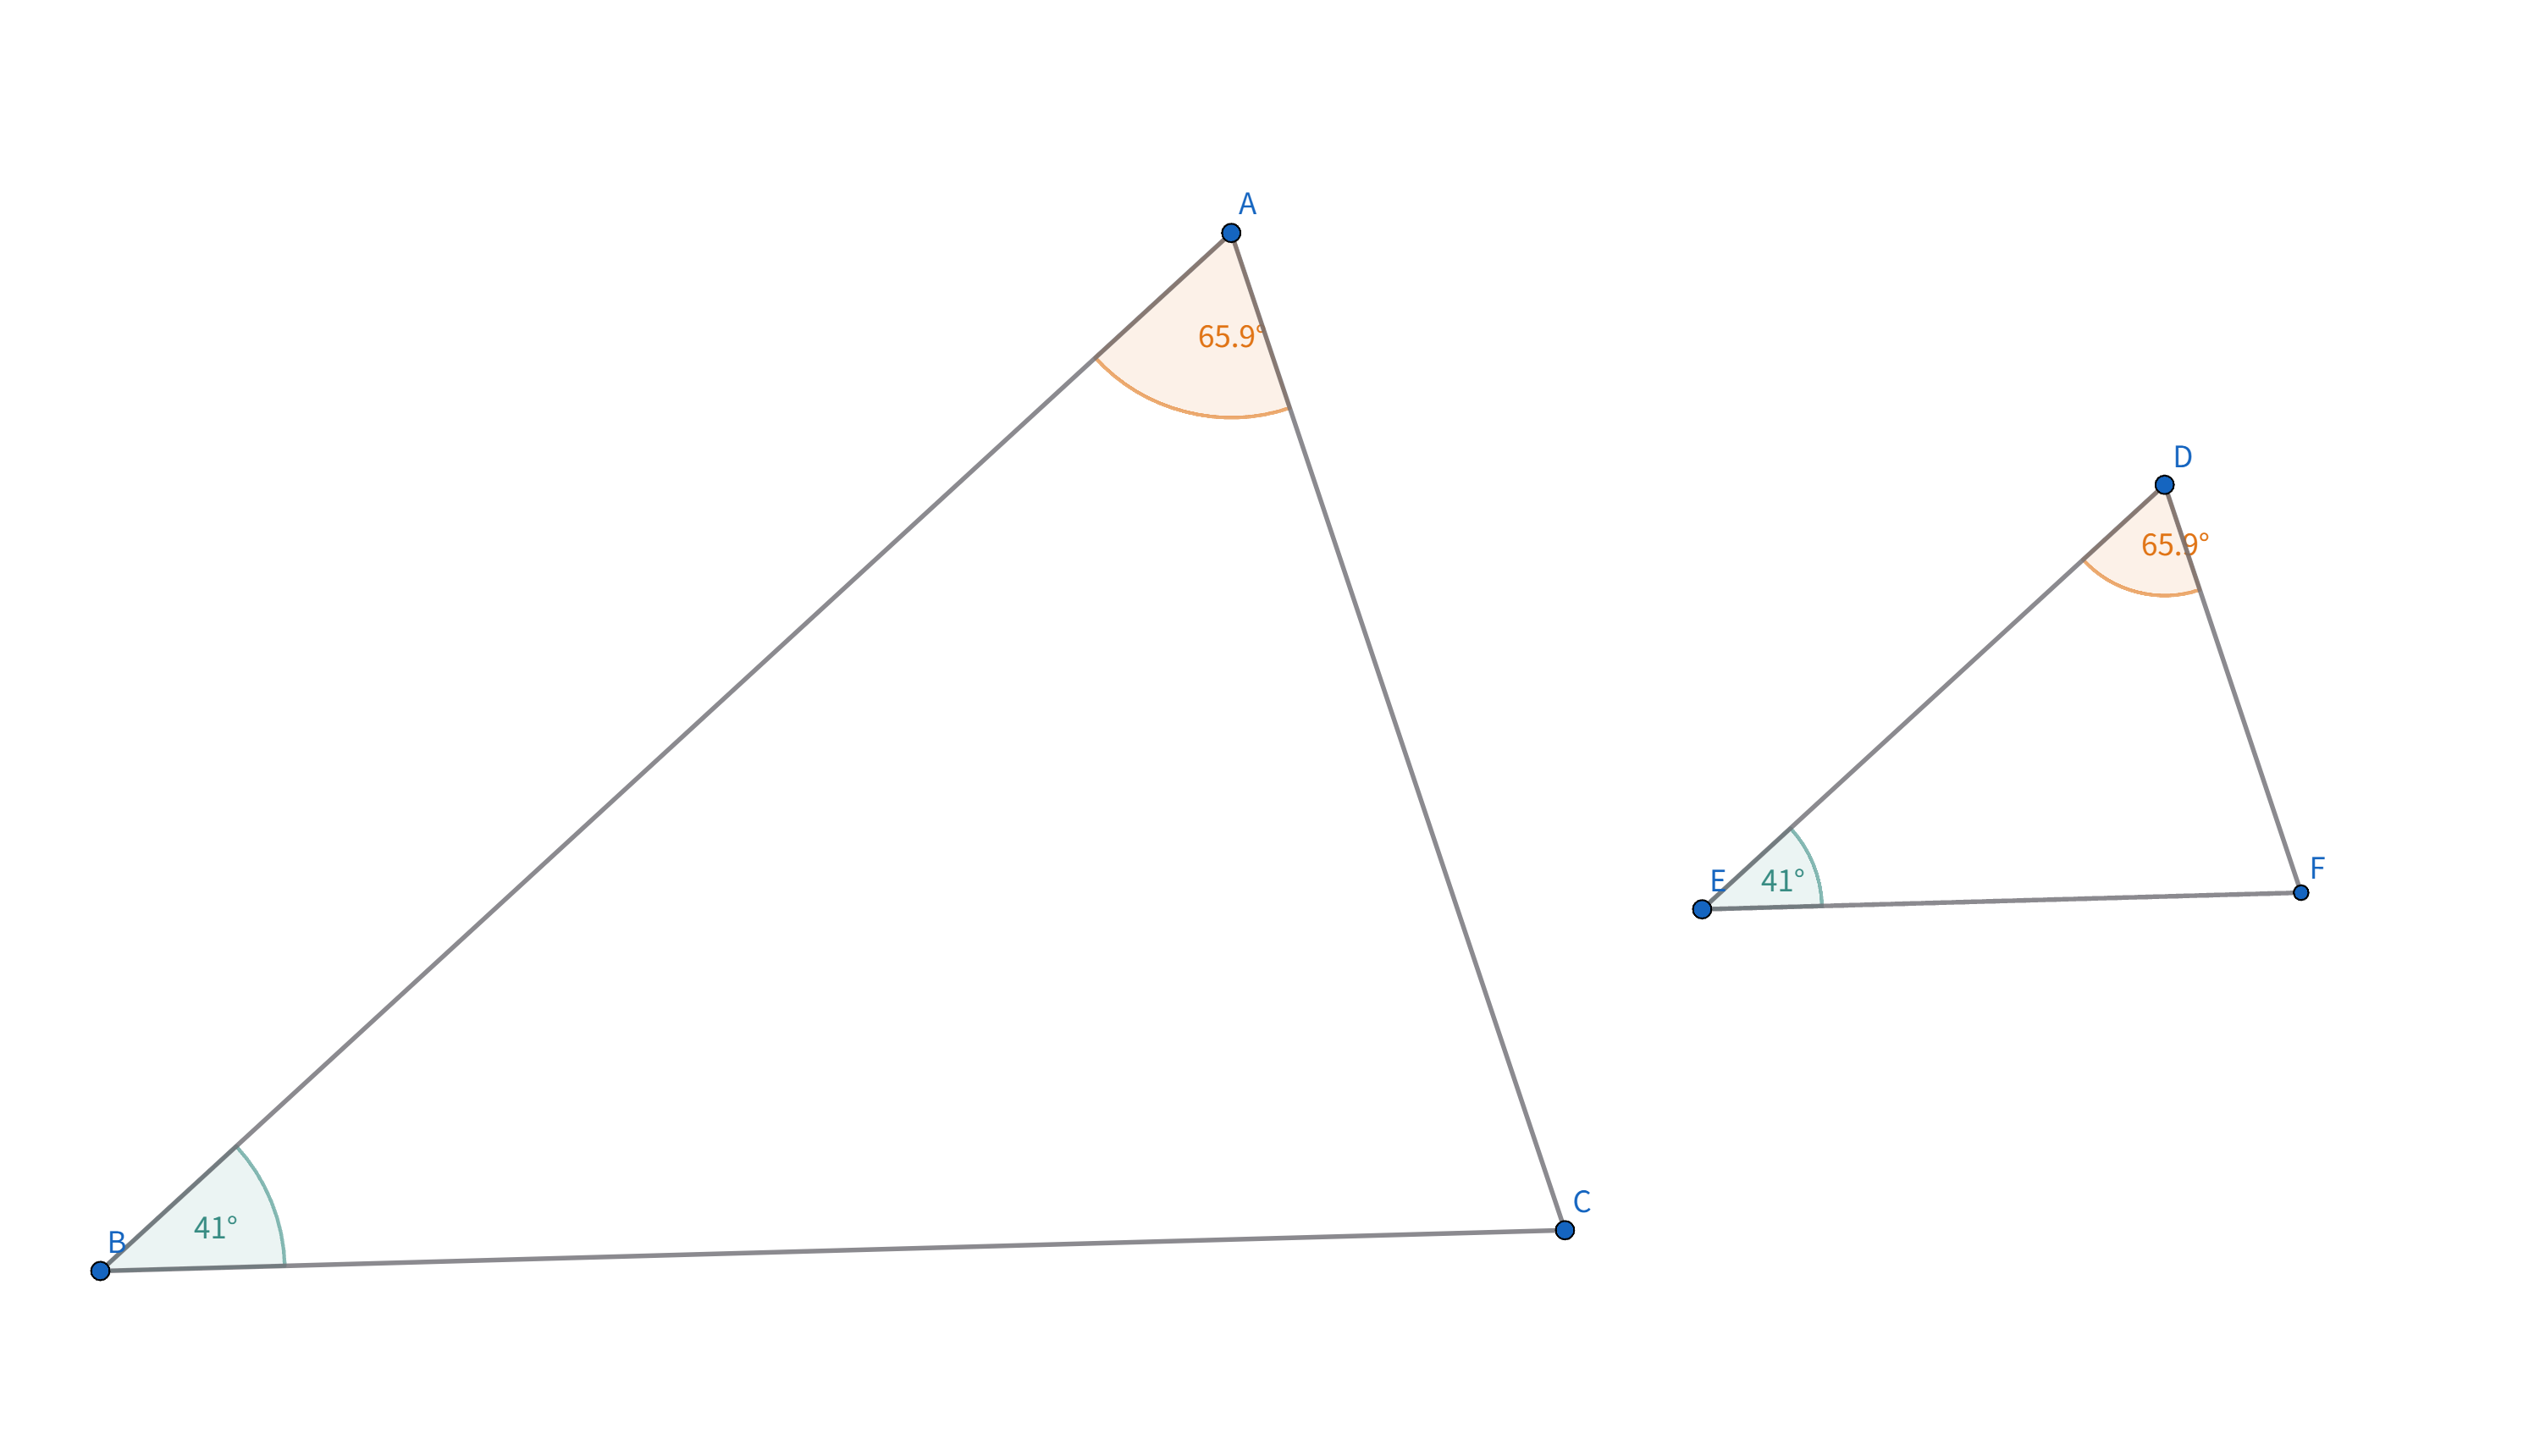
\includegraphics[width=\linewidth]{figures/AA相似.png}
        \caption{AA相似}
        % \label{fig:side:b}
    \end{minipage}
    \hfill % 添加一些水平间距
    \begin{minipage}[t]{0.3\textwidth}
    \centering
    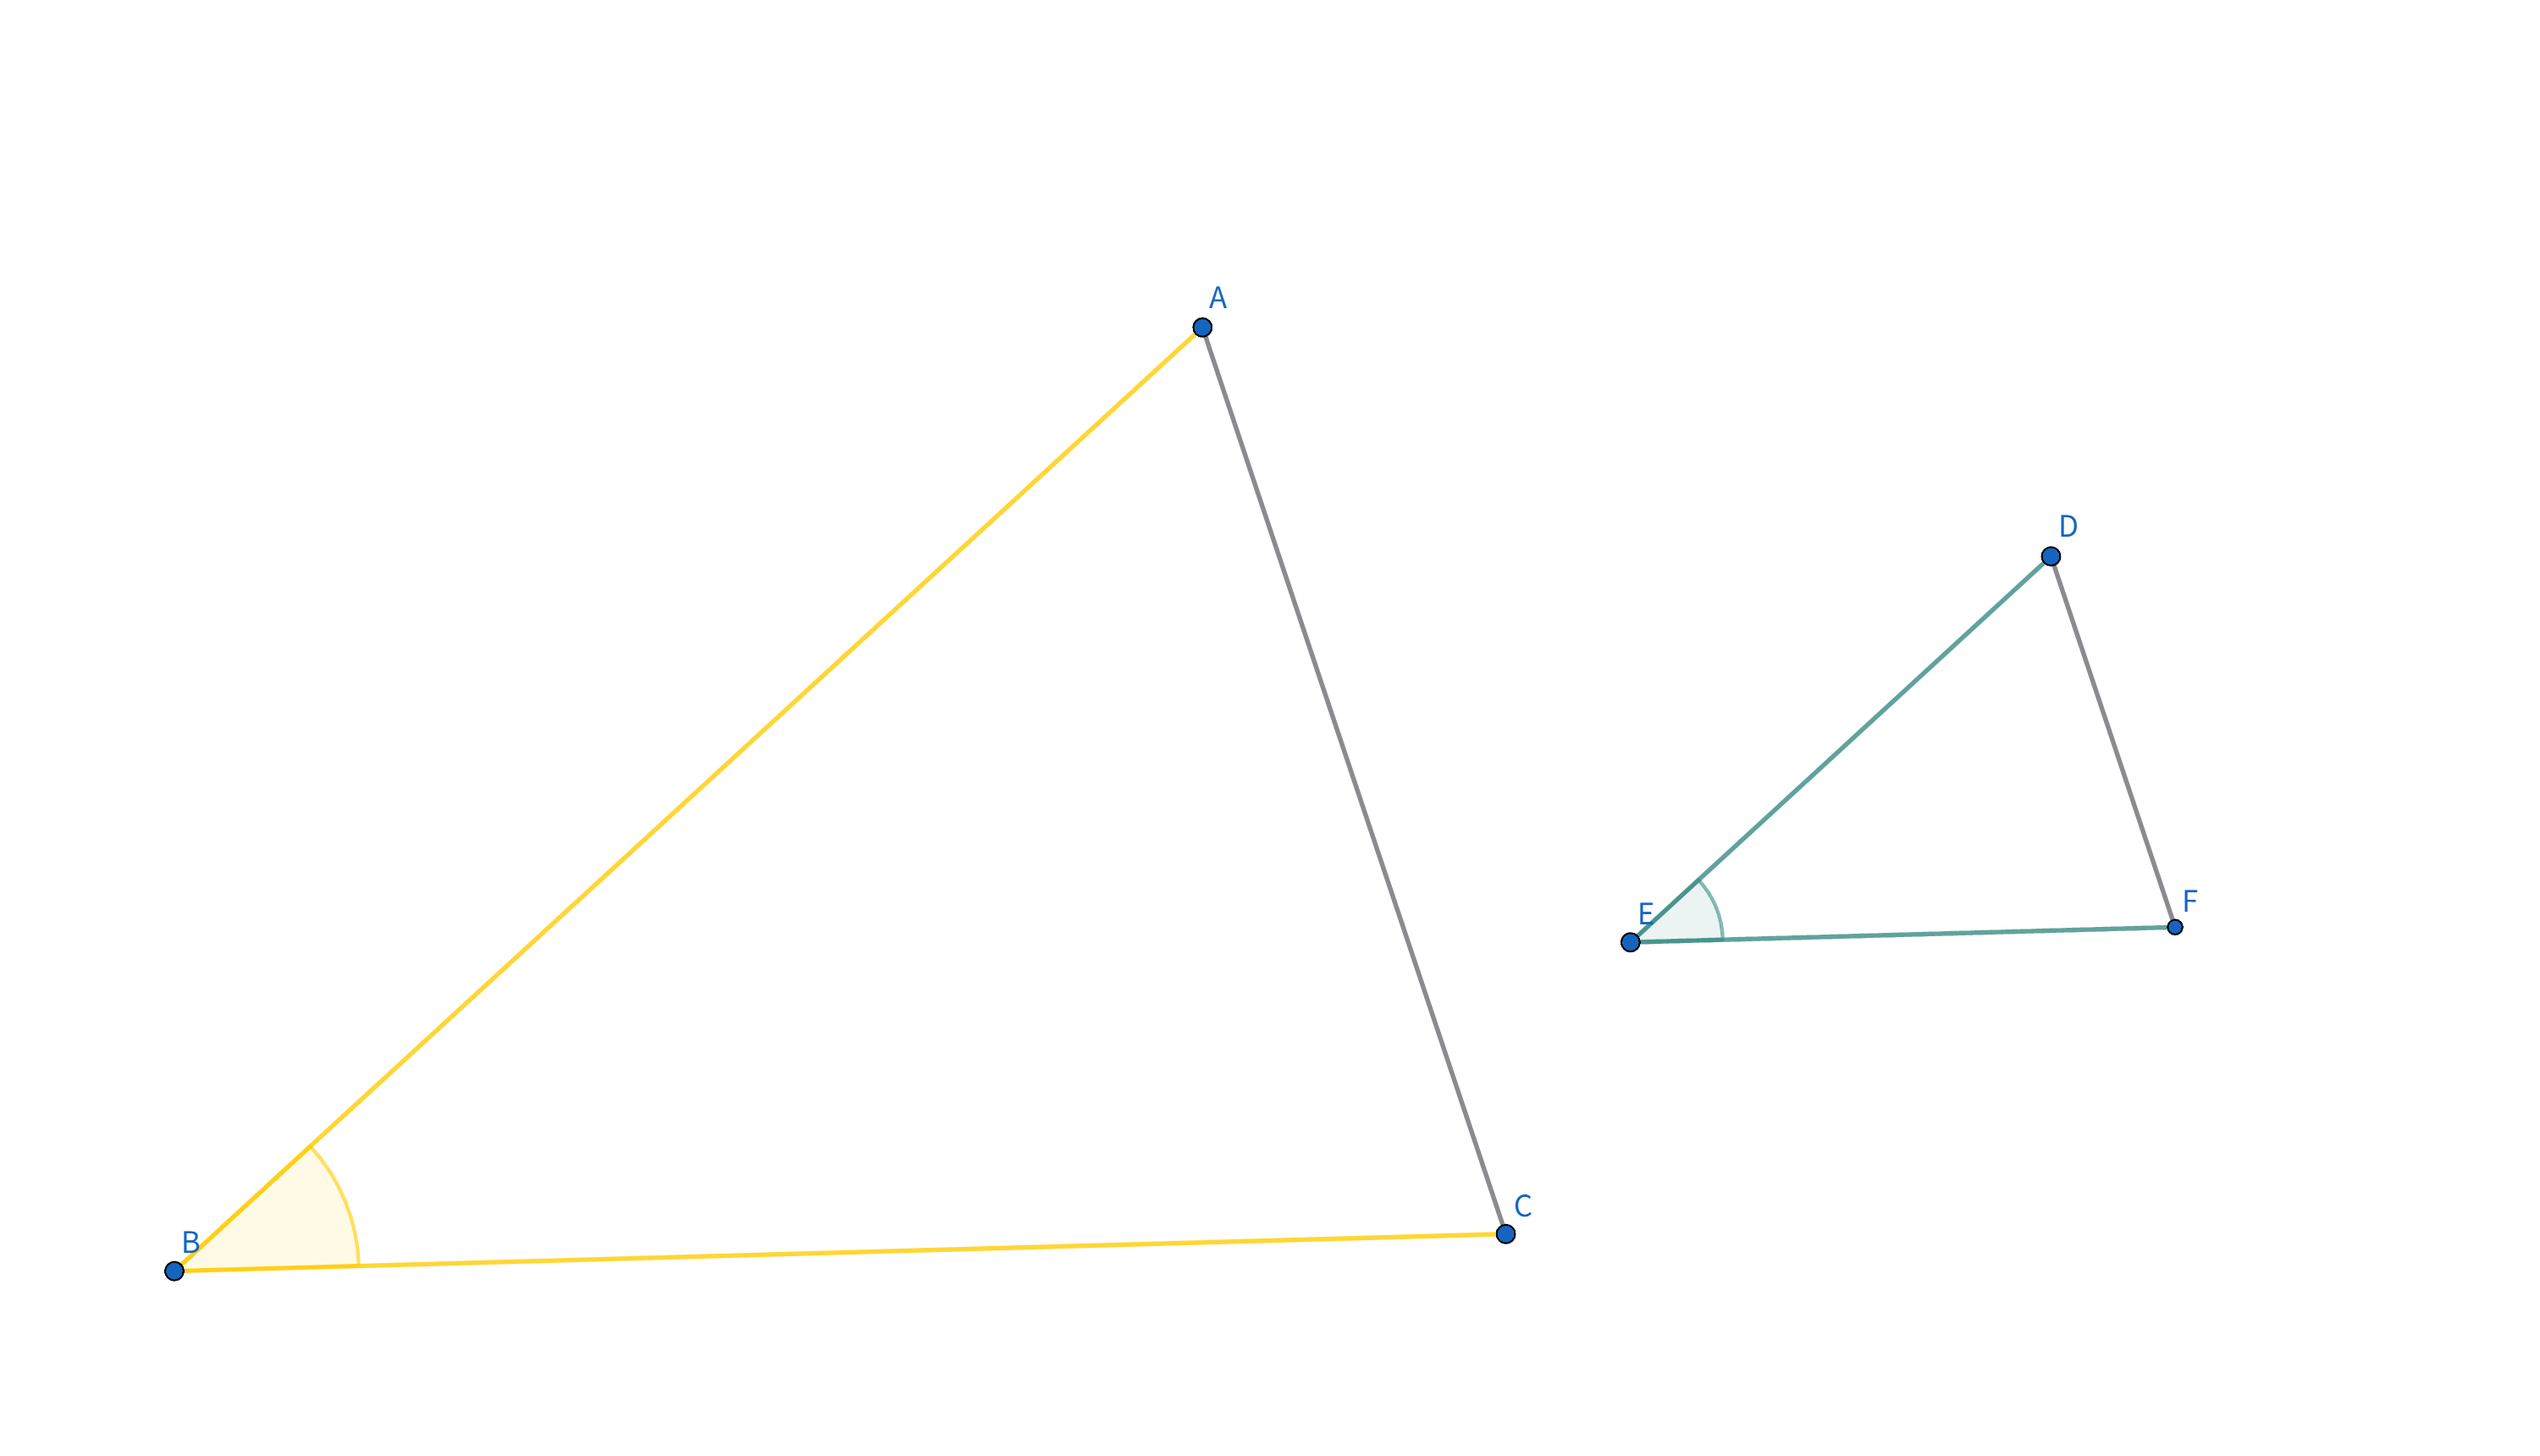
\includegraphics[width=\linewidth]{figures/SAS相似.png}
    \caption{SAS相似}
    \end{minipage}
    \begin{minipage}[t]{0.3\textwidth}
    \centering
    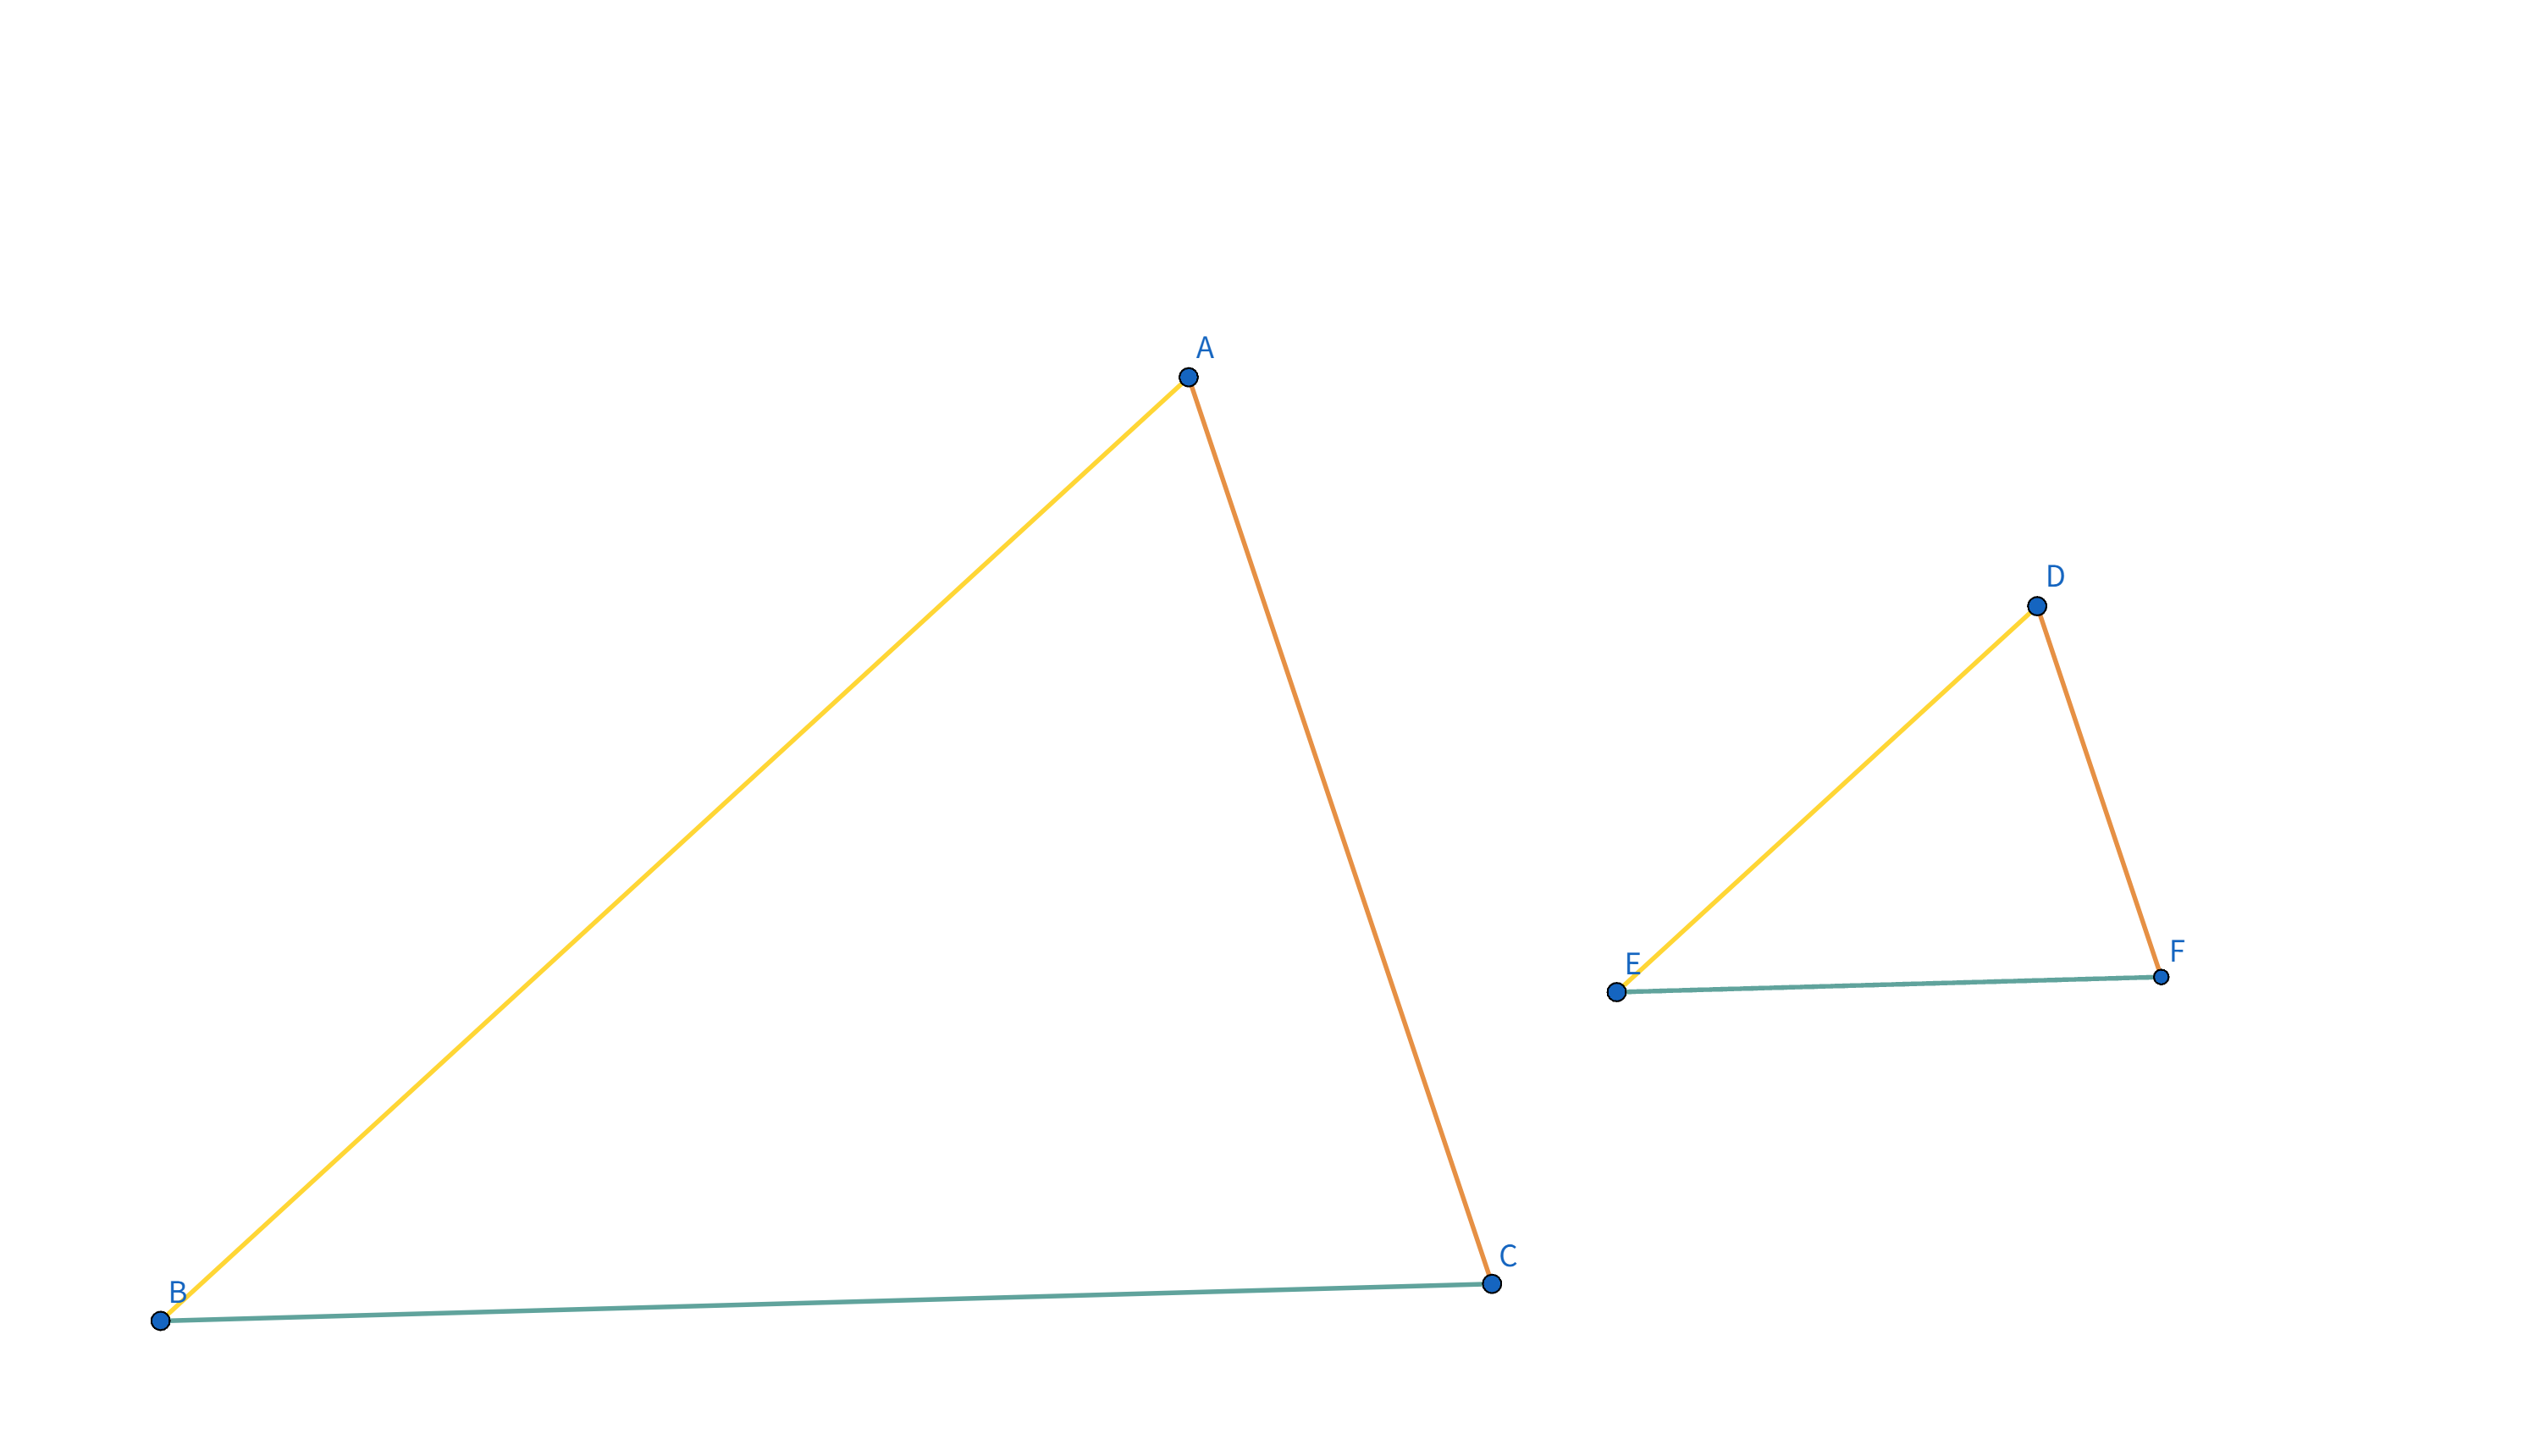
\includegraphics[width=\linewidth]{figures/SSS相似.png}
    \caption{SSS相似}
    \end{minipage}
\end{figure}












\subsection{常见形式}

\begin{figure}[h]
    \centering
    \hfill % 添加一些水平间距
    \begin{minipage}[t]{0.45\textwidth}
    \centering
    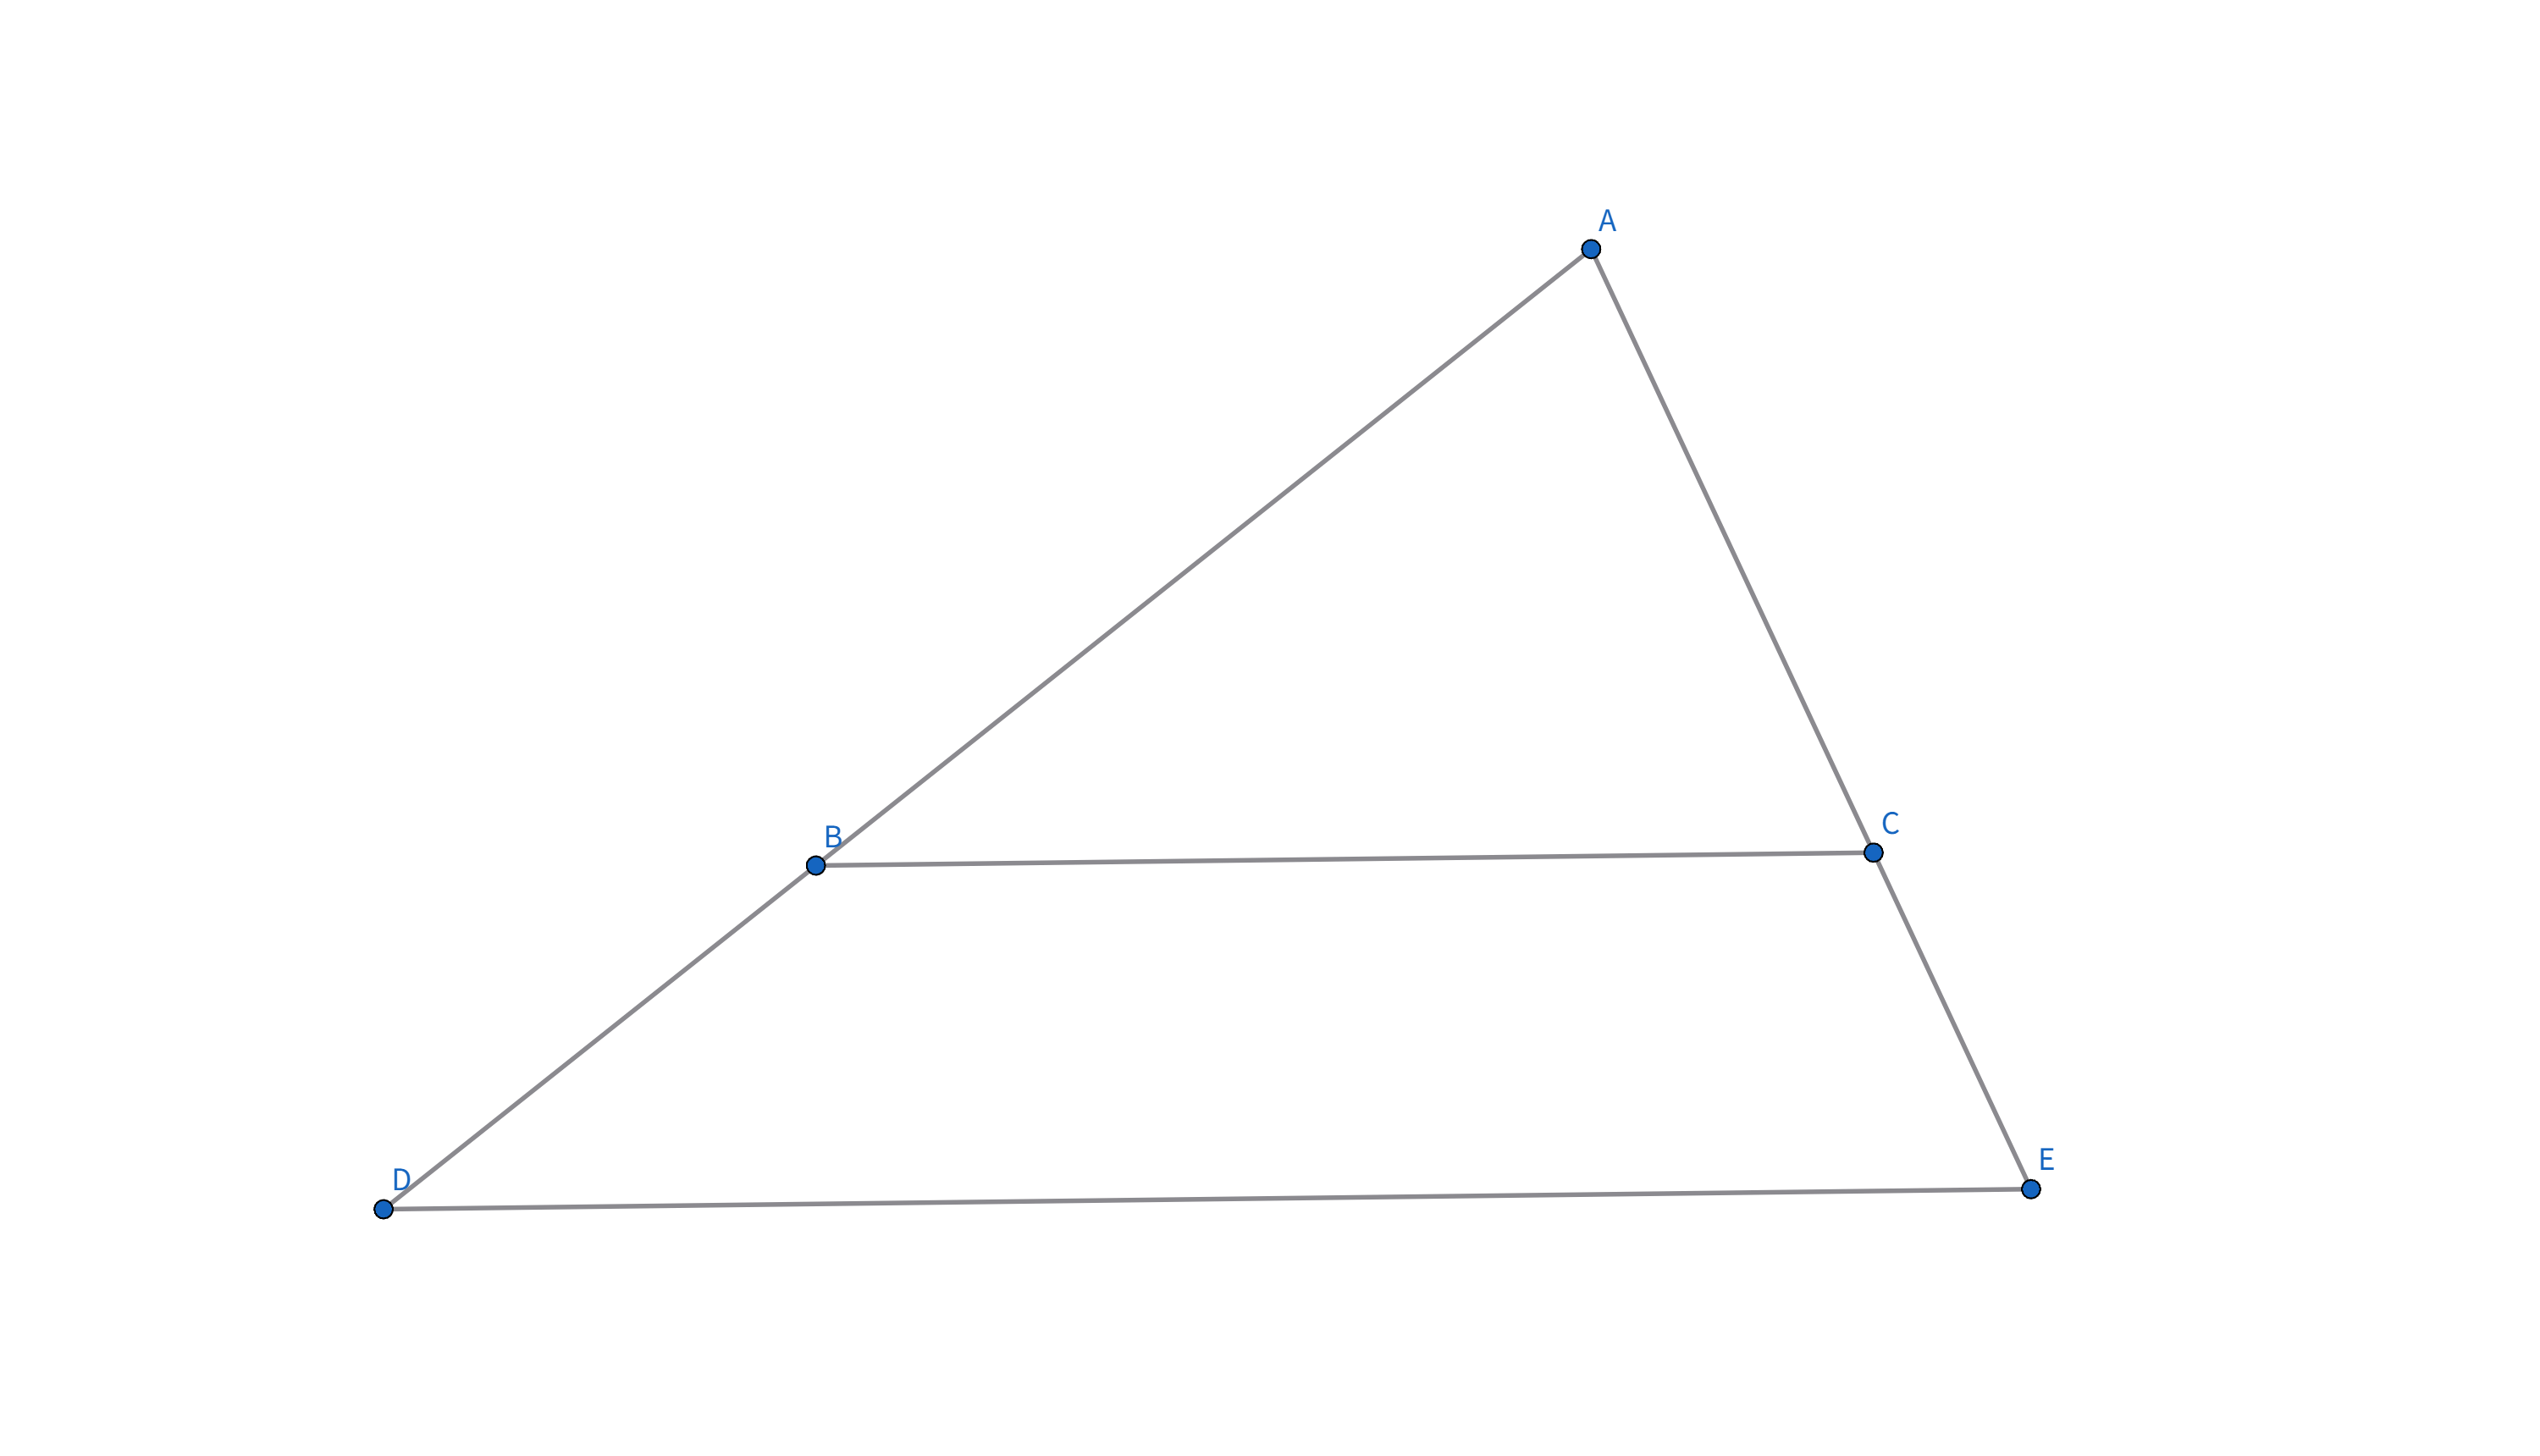
\includegraphics[width=0.8\linewidth]{figures/平行相似.png}
    \caption{平行相似}
    \end{minipage}
    \hfill % 添加一些水平间距
    \begin{minipage}[t]{0.45\textwidth}
    \centering
    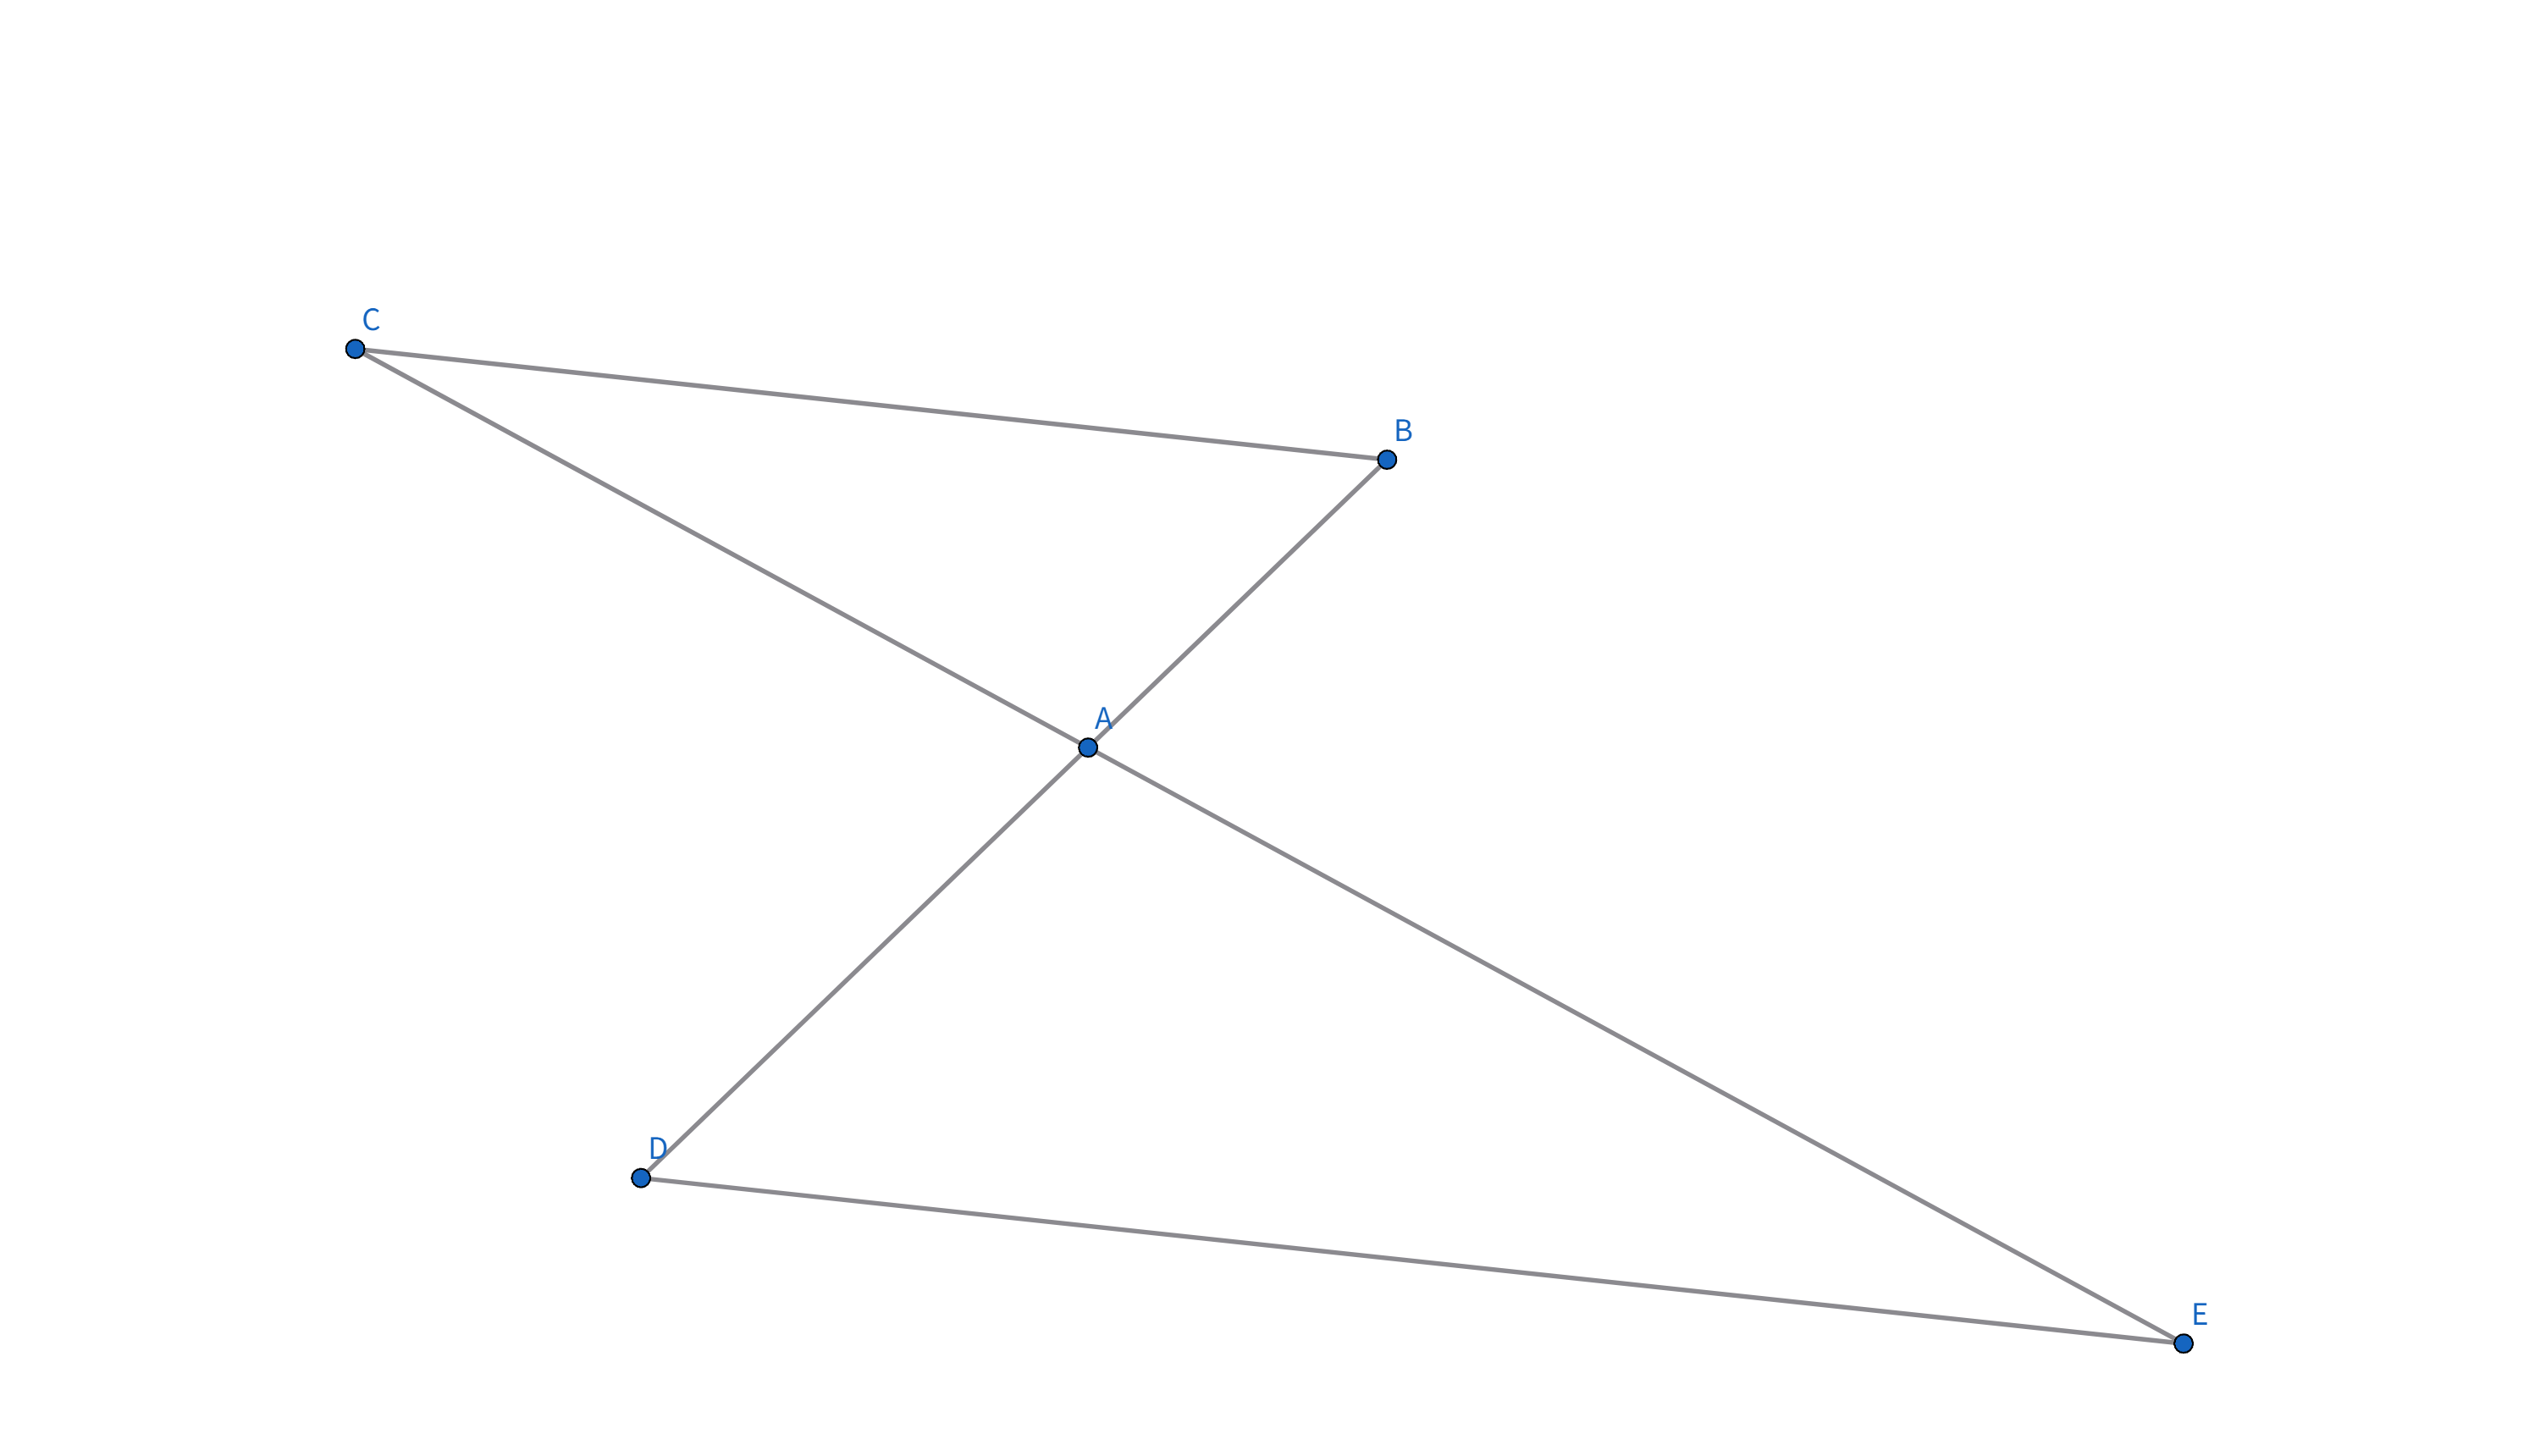
\includegraphics[width=0.8\linewidth]{figures/平行相似2.png}
    \caption{平行相似}
    \end{minipage}
\end{figure}

\begin{figure}[h]
    \centering
    \hfill % 添加一些水平间距
    \begin{minipage}[t]{0.45\textwidth}
    \centering
    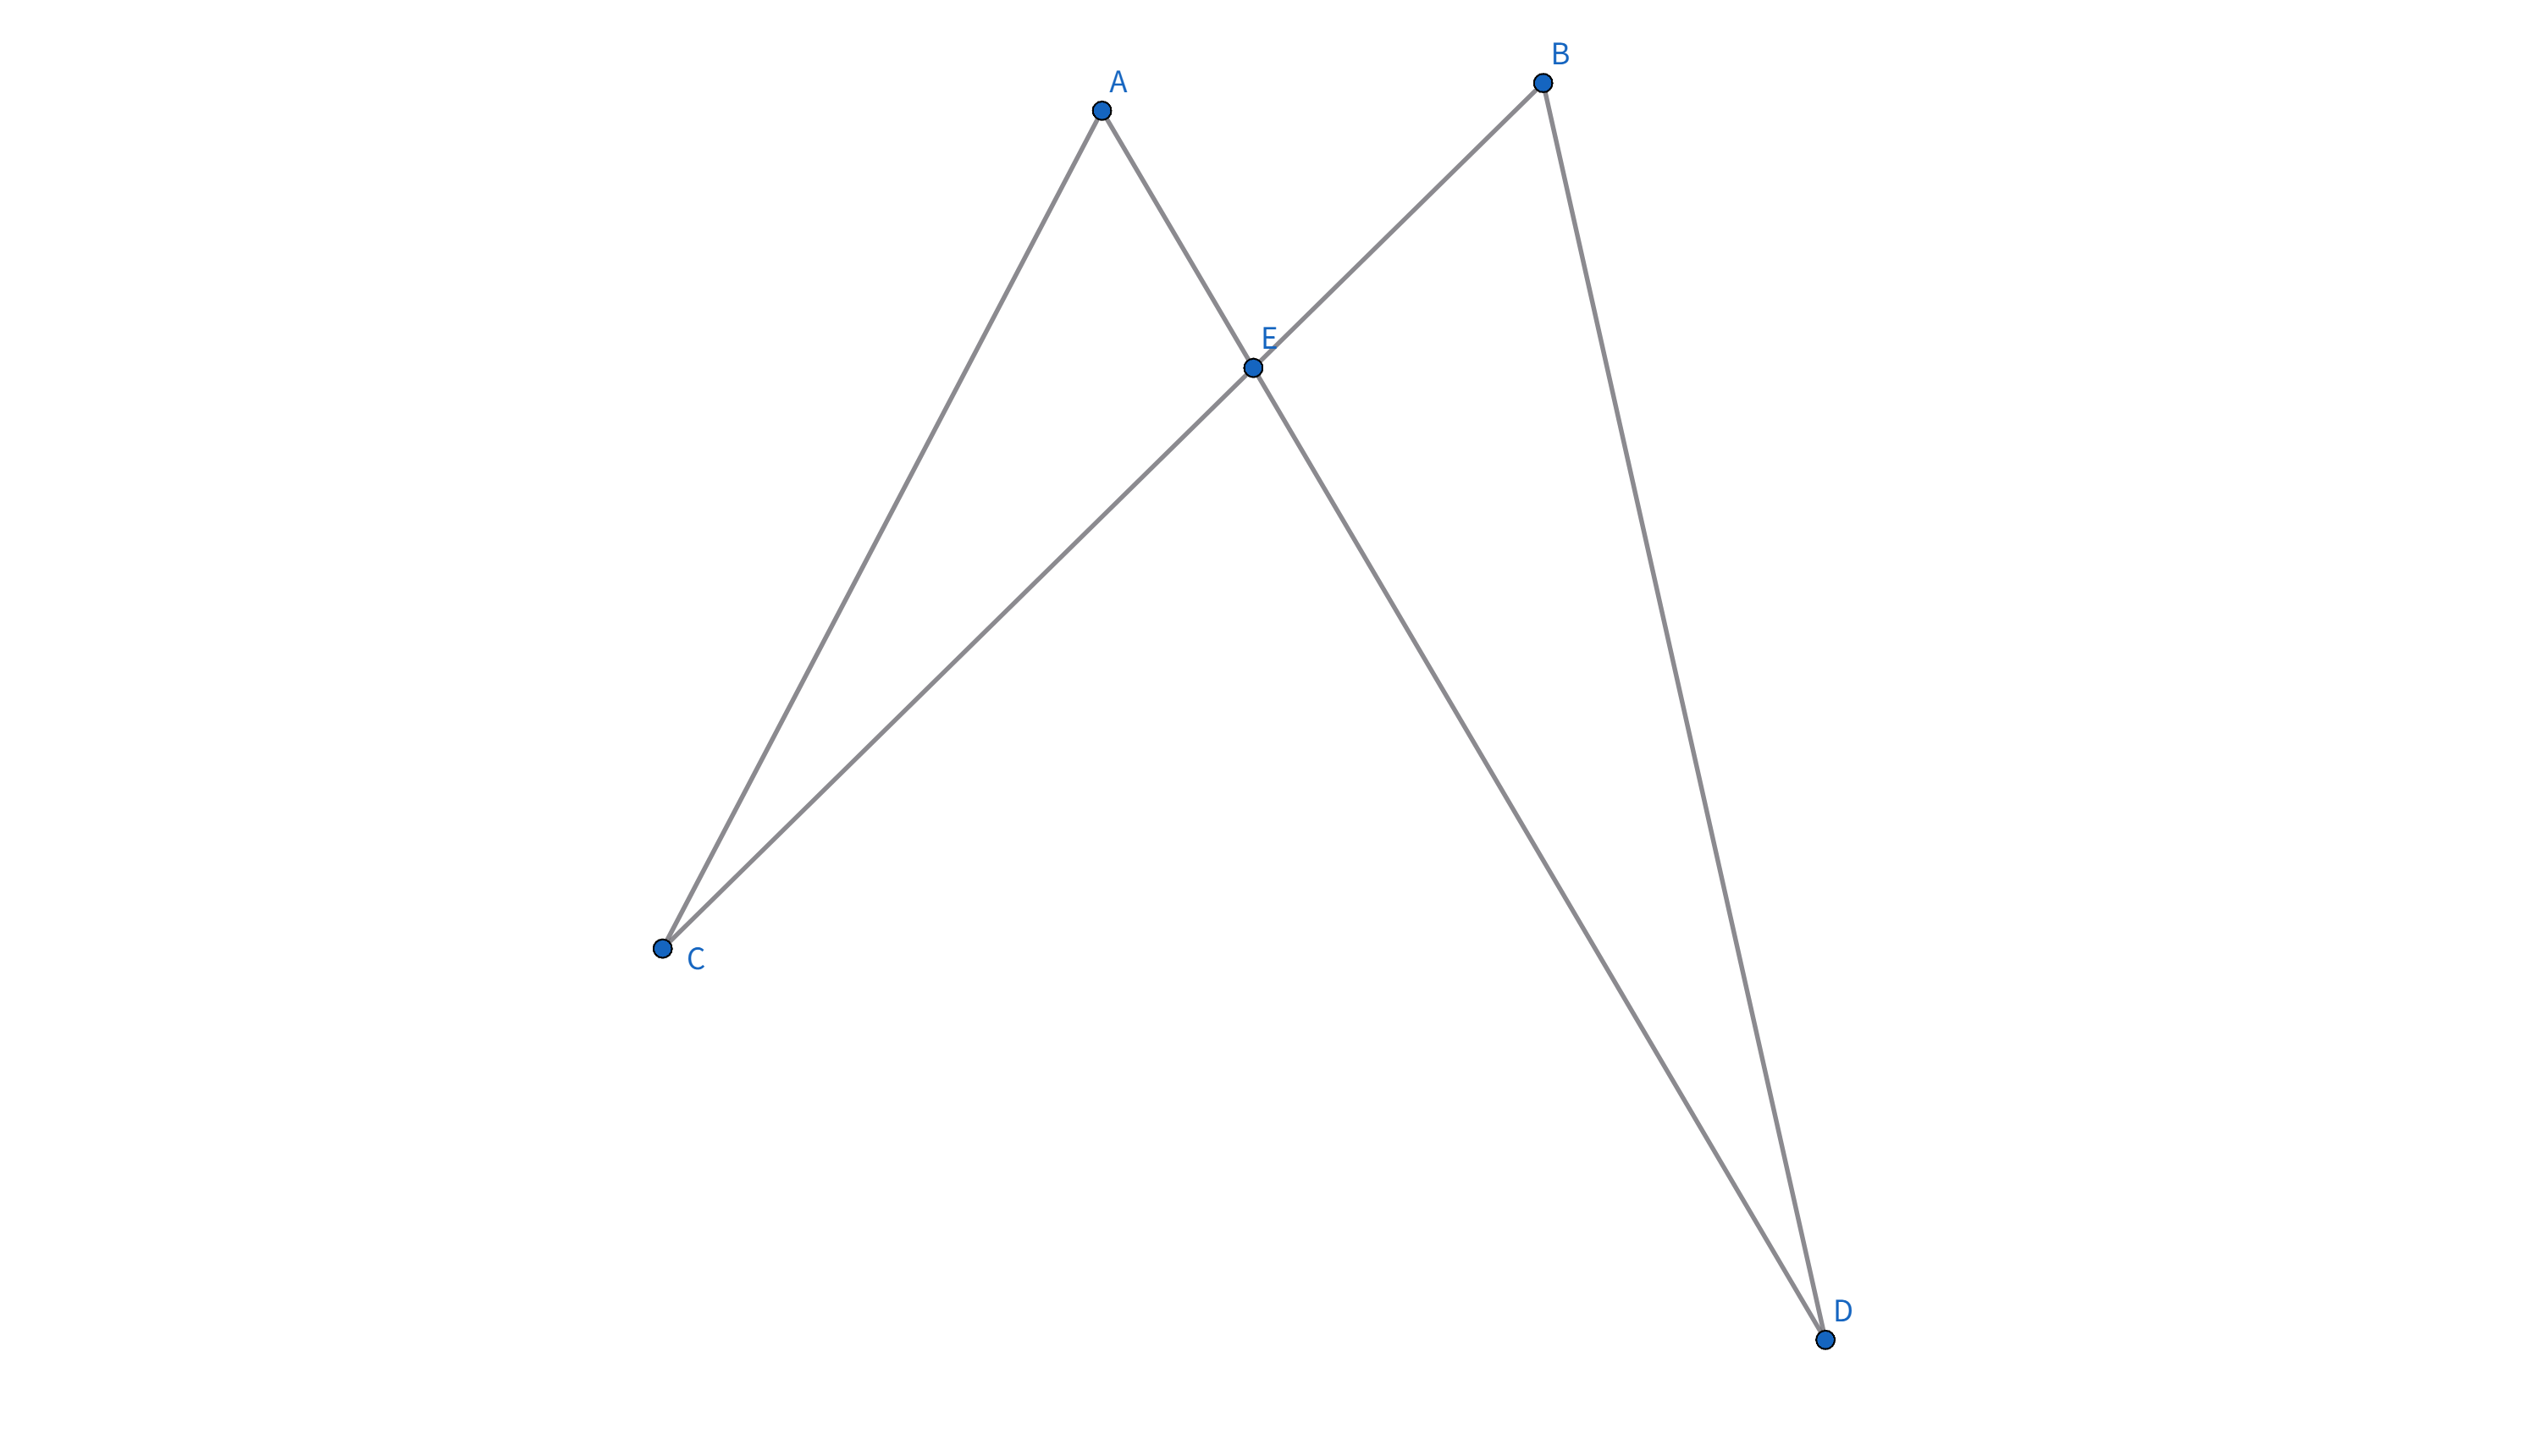
\includegraphics[width=0.8\linewidth]{figures/蝴蝶型相似.png}
    \caption{蝴蝶型相似}
    \end{minipage}
    \hfill % 添加一些水平间距
    \begin{minipage}[t]{0.45\textwidth}
    \centering
    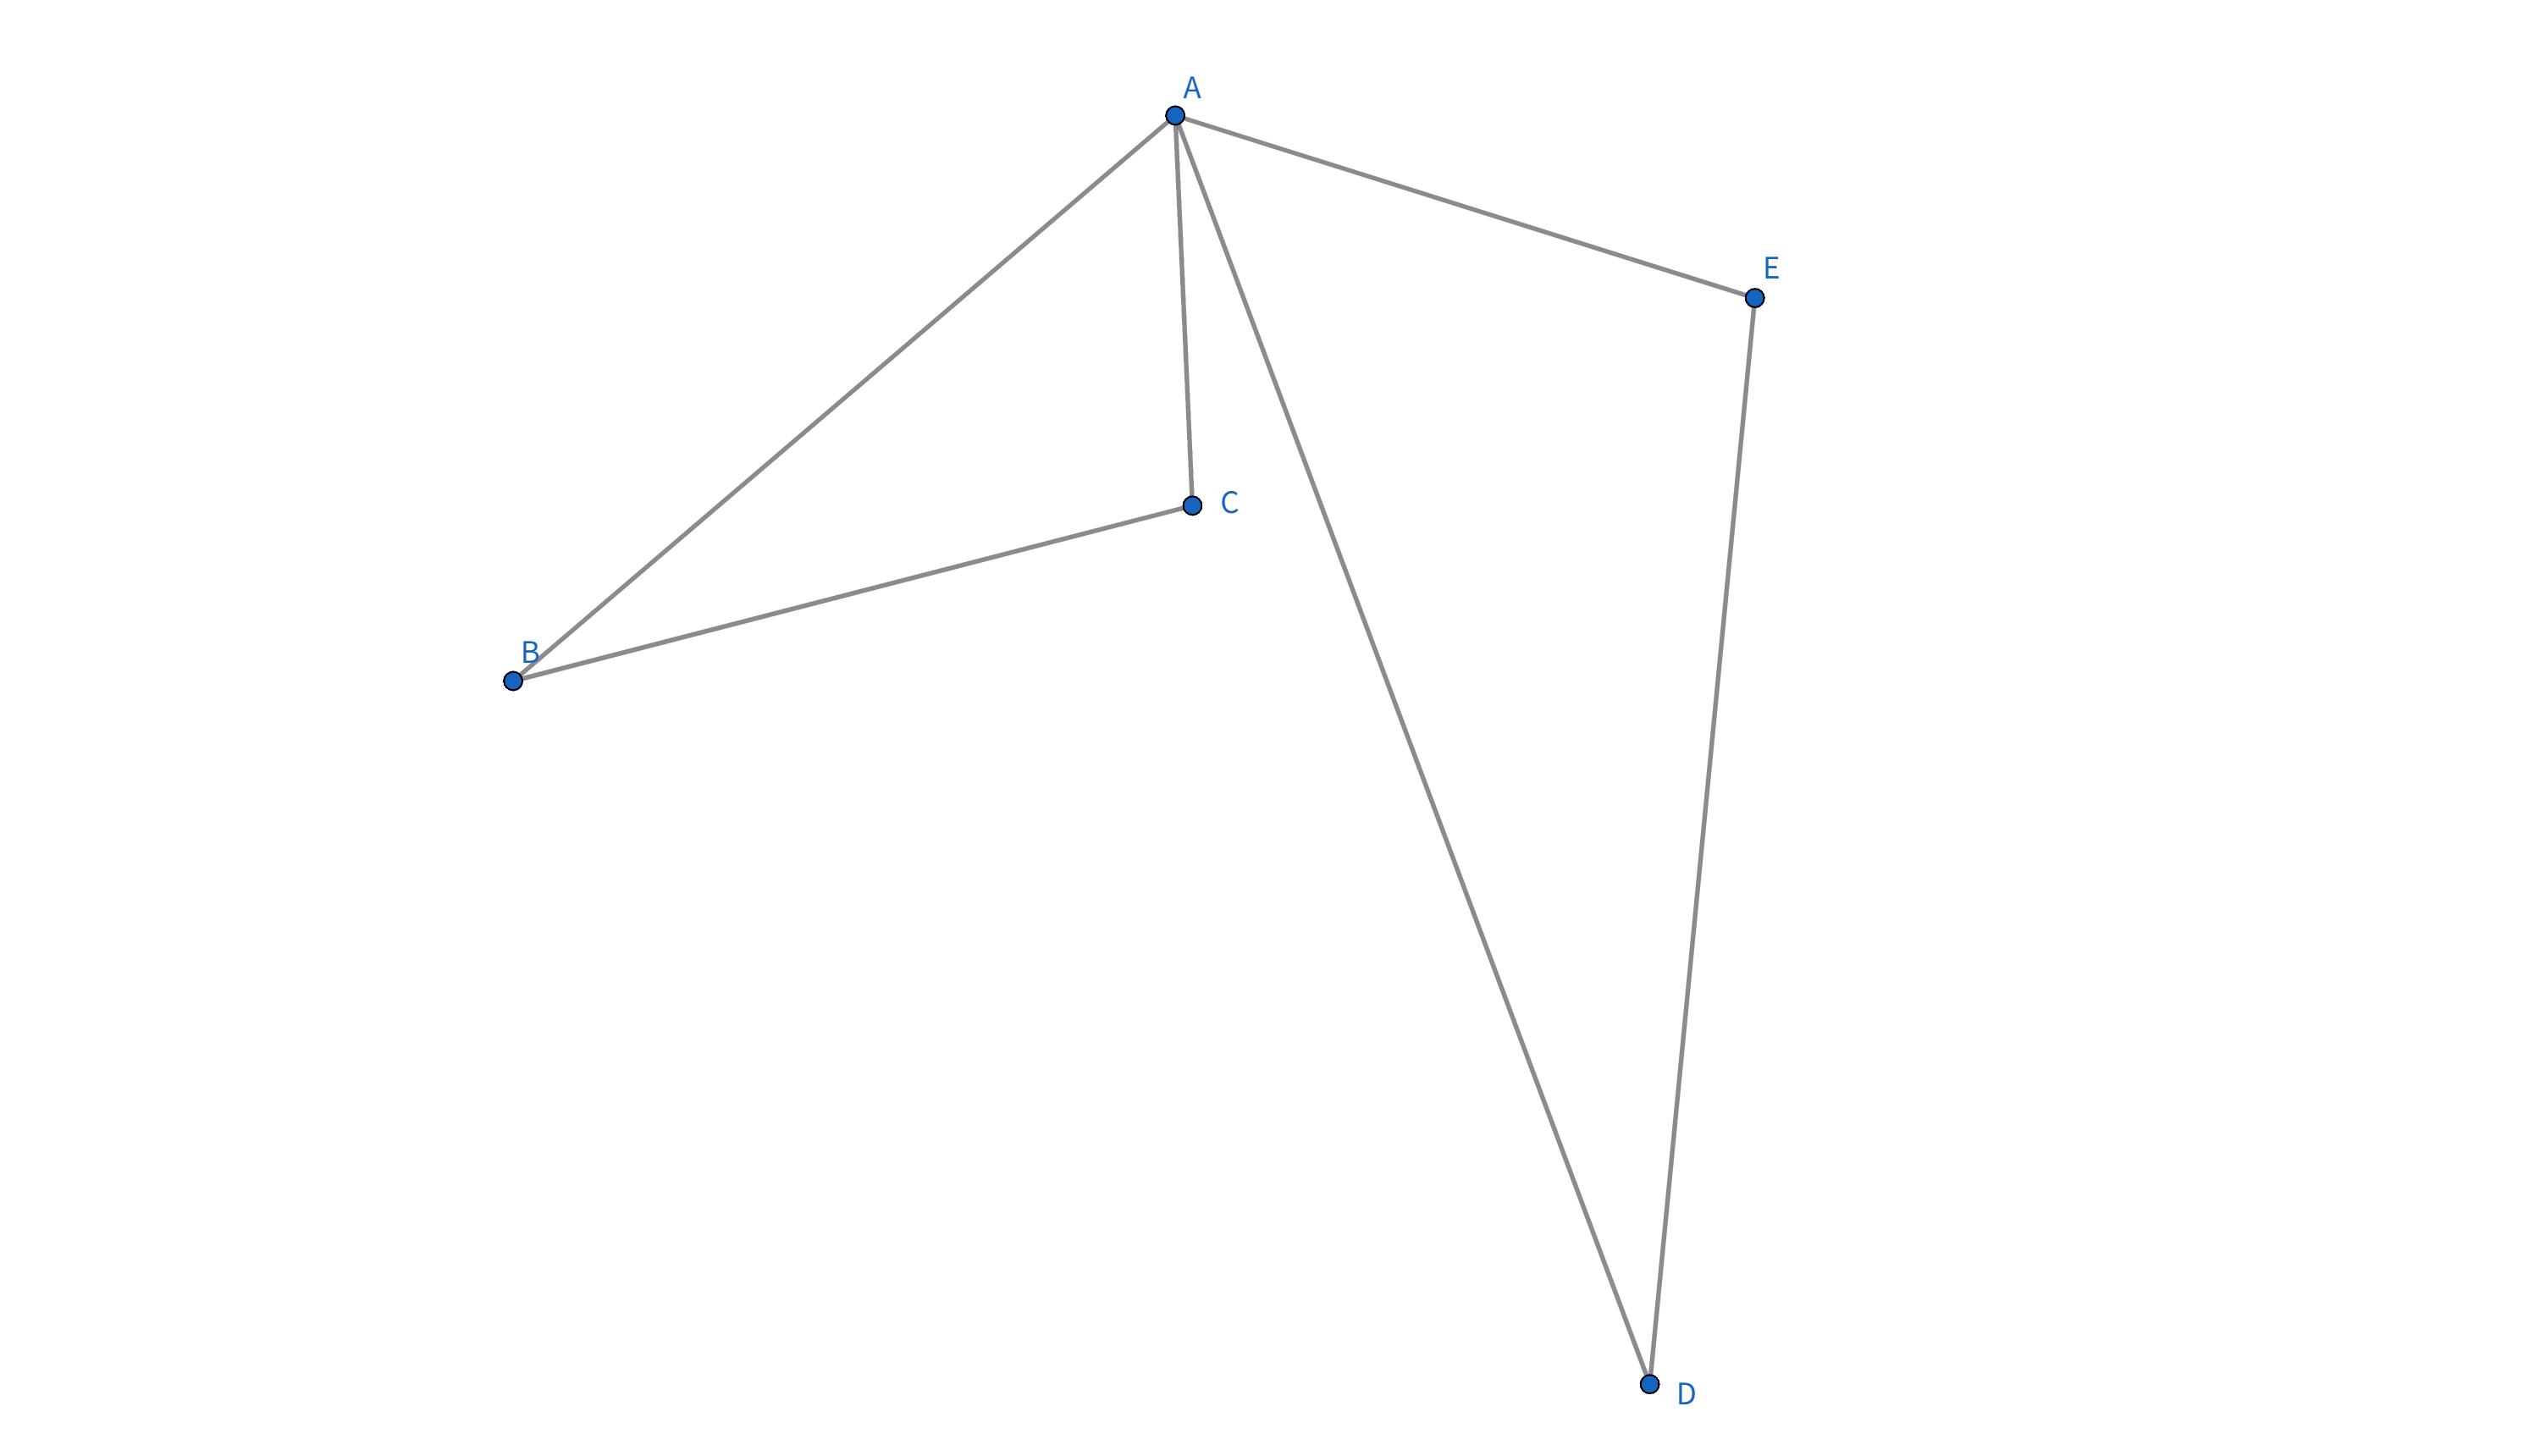
\includegraphics[width=0.8\linewidth]{figures/旋转型相似.png}
    \caption{旋转型相似}
    \end{minipage}
\end{figure}


\begin{figure}[h]
    \centering
    \hfill % 添加一些水平间距
    \begin{minipage}[t]{0.45\textwidth}
    \centering
    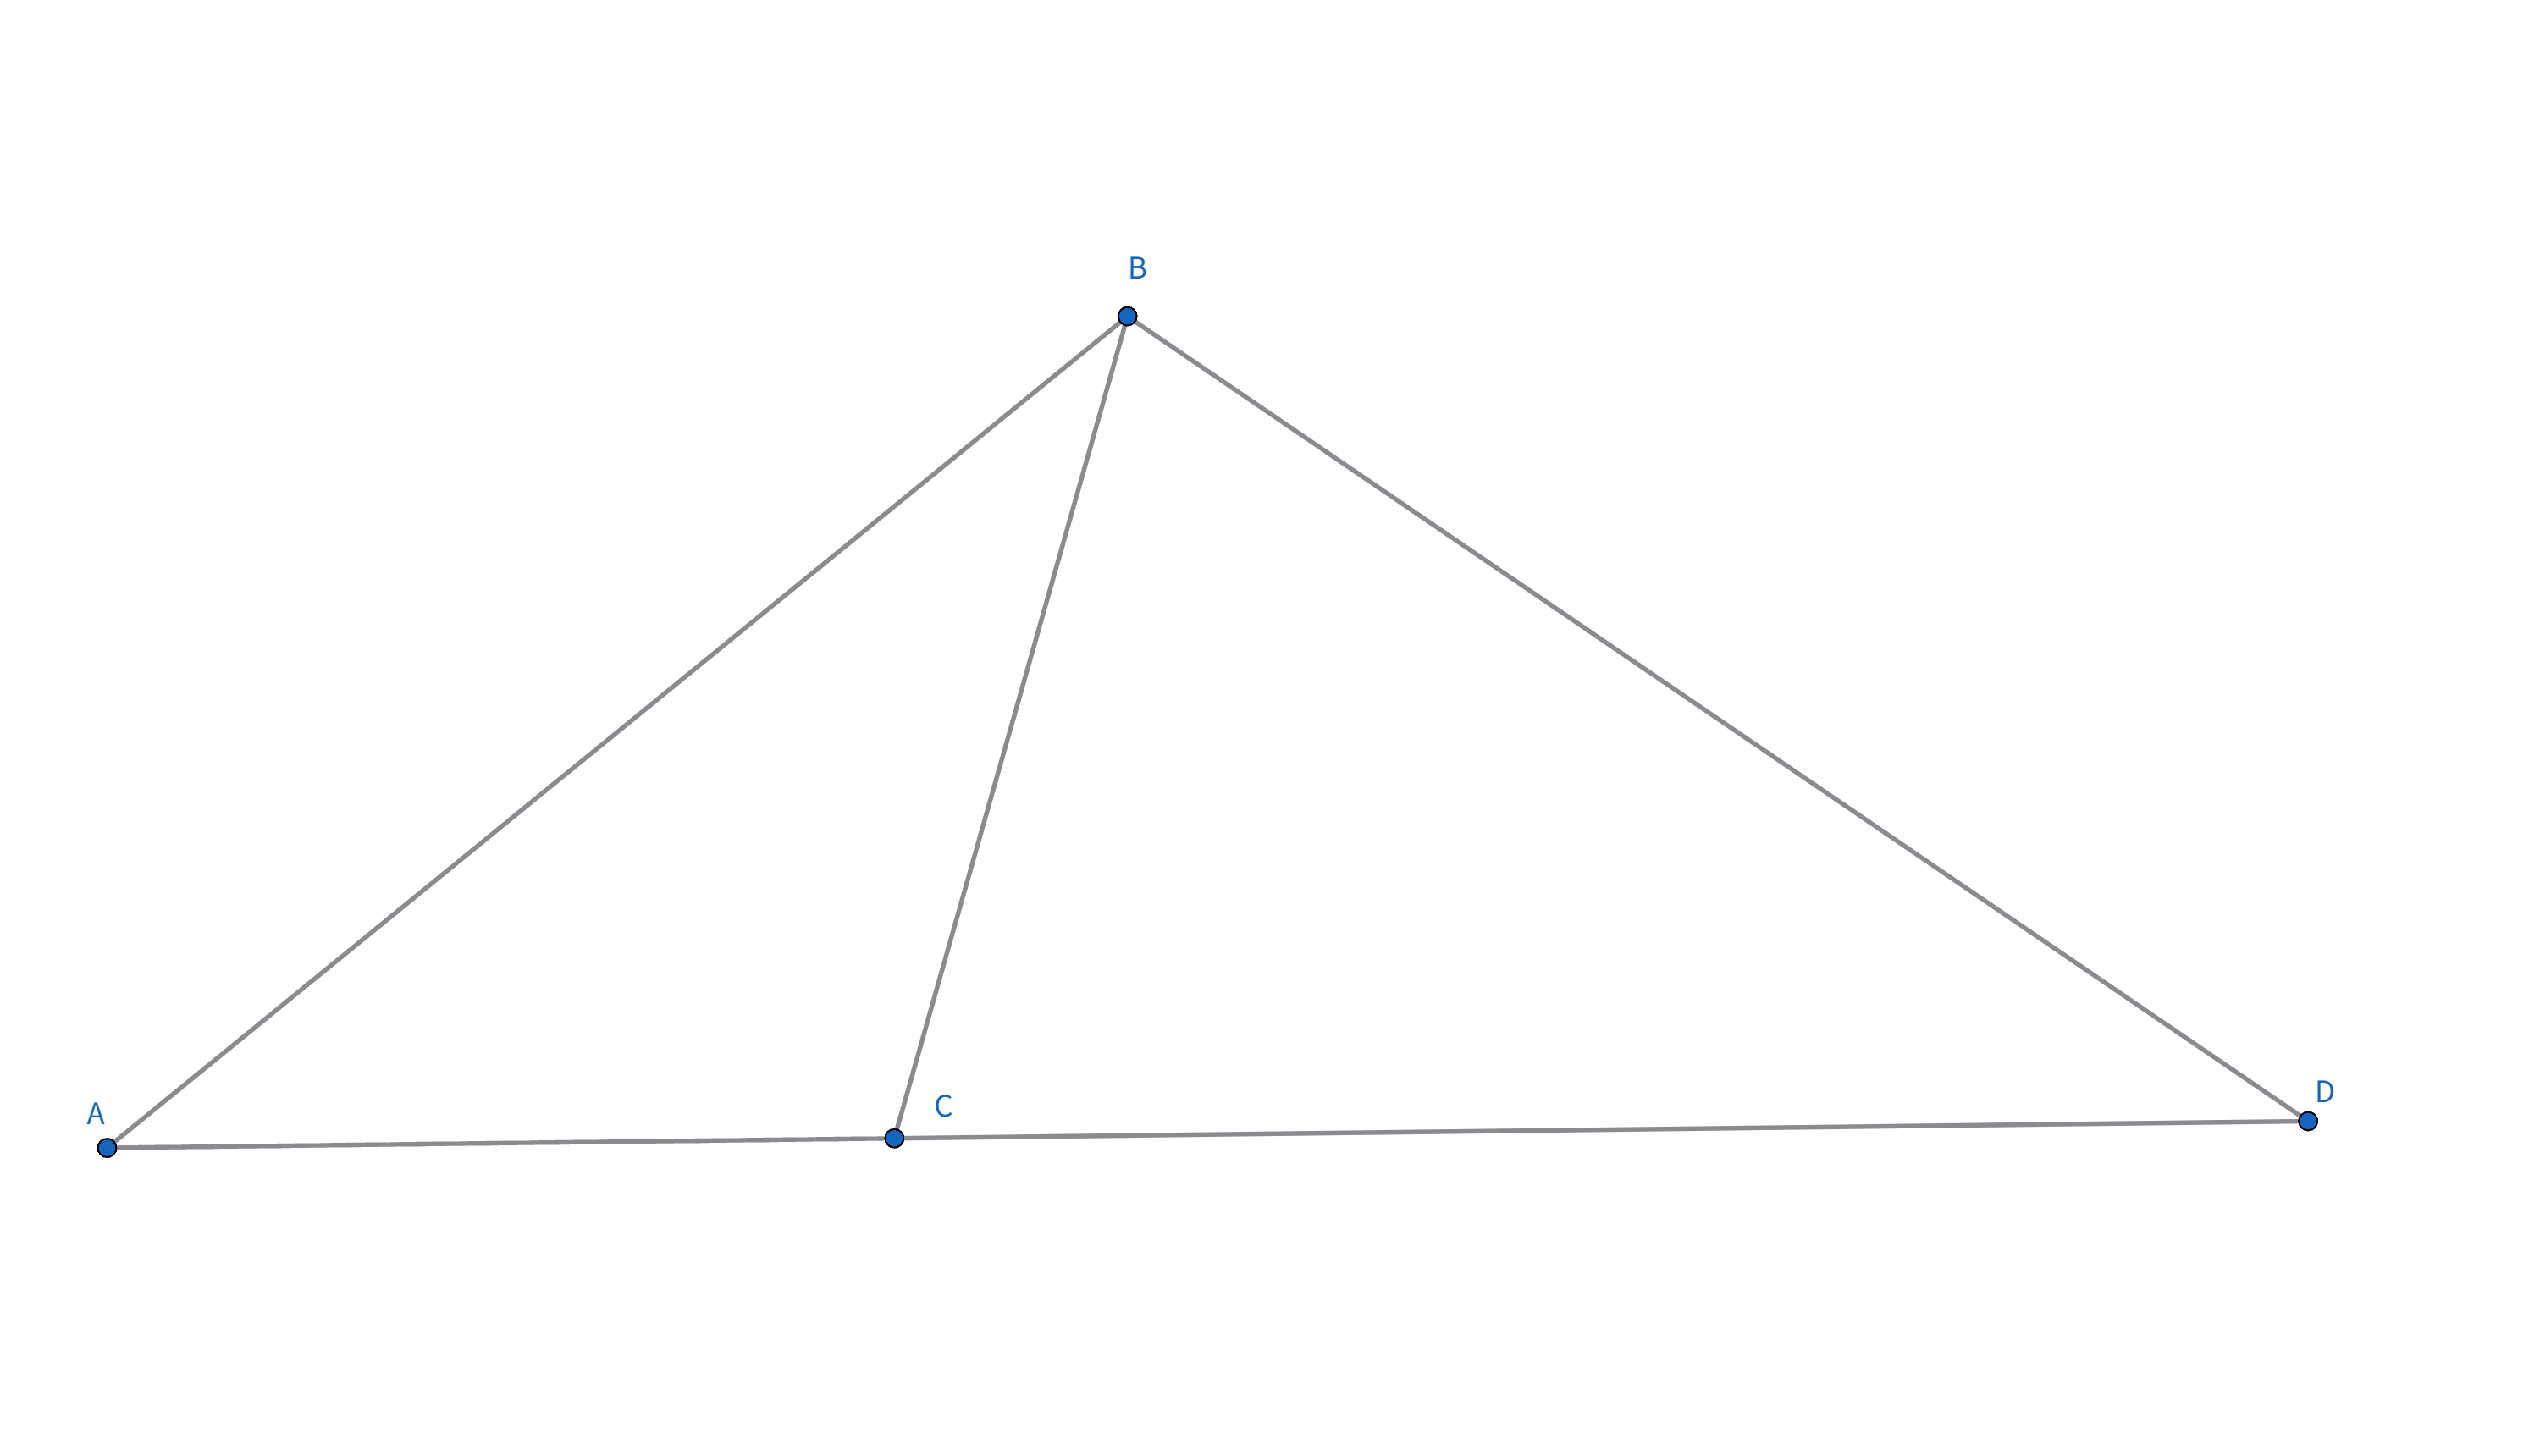
\includegraphics[width=0.8\linewidth]{figures/子母型相似.png}
    \caption{子母型相似}
    \end{minipage}
    \hfill % 添加一些水平间距
    \begin{minipage}[t]{0.45\textwidth}
    \centering
    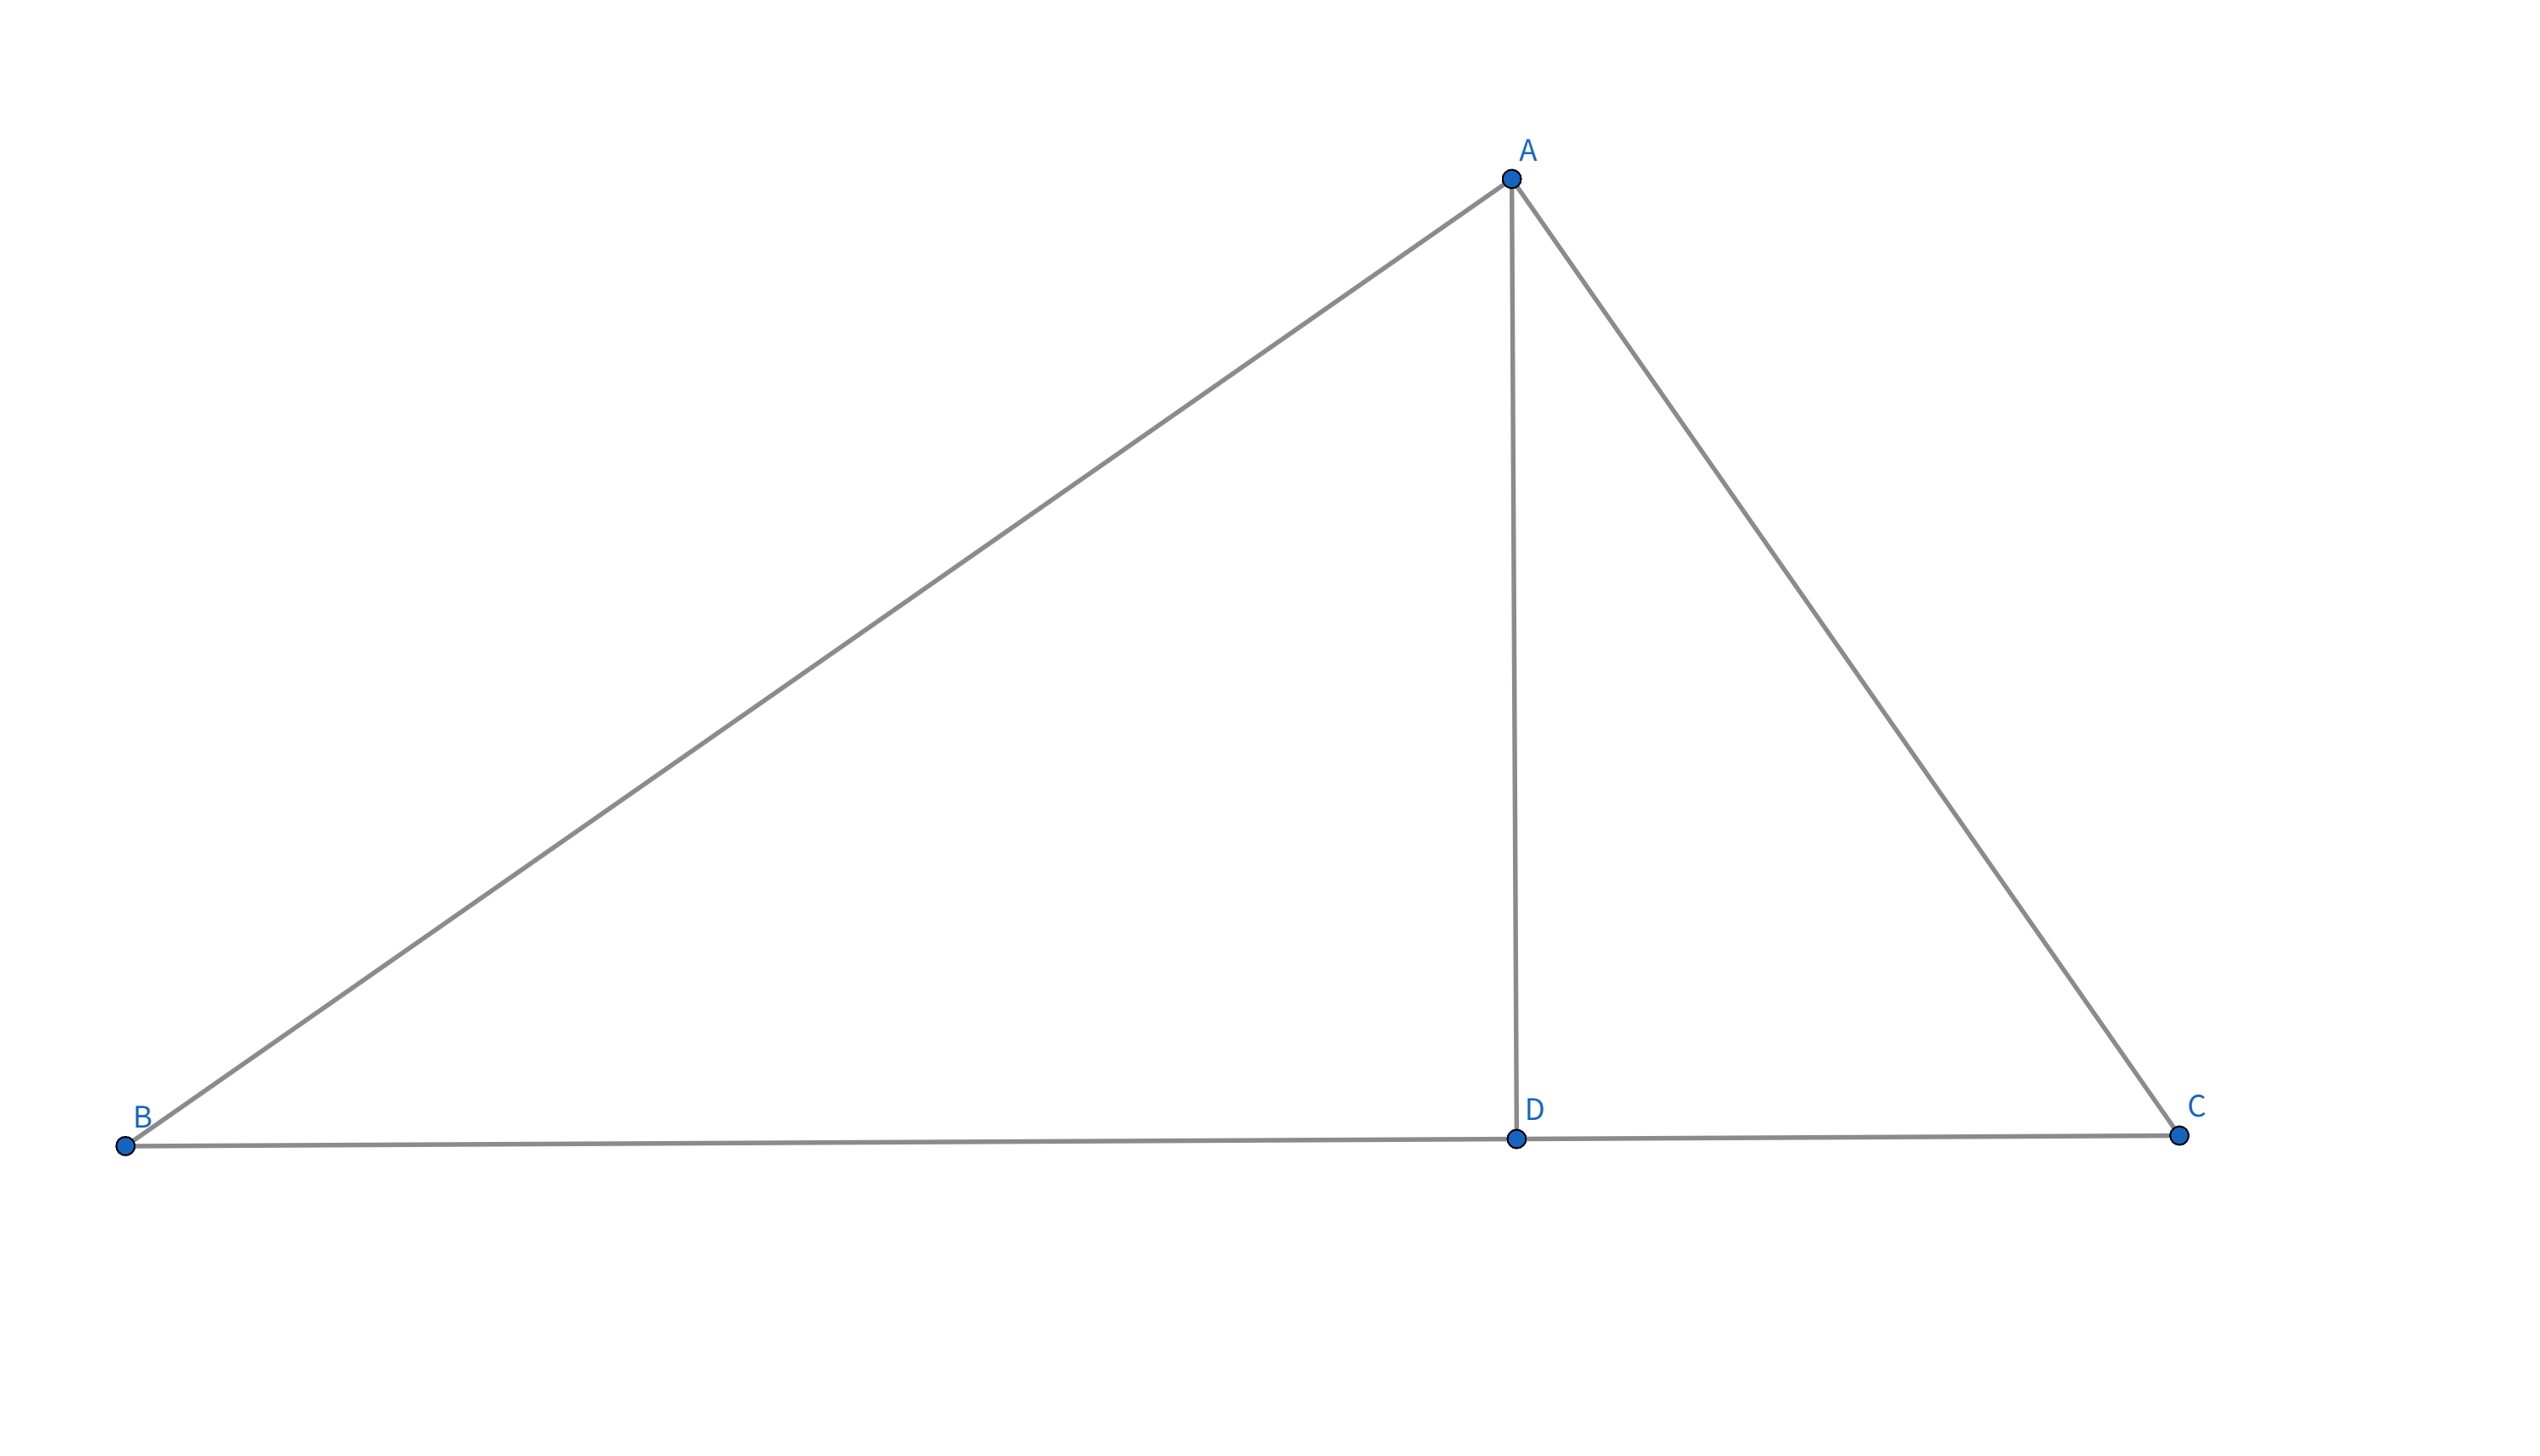
\includegraphics[width=0.8\linewidth]{figures/射影定理.png}
    \caption{直角子母型相似}
    \end{minipage}
\end{figure}




\subsection{射影定理}
\begin{theorem}[射影定理]
    在直角$\triangle ABC$中,AD为斜边BC上的垂线,D为垂足。有下面等式成立:
    $$
    \begin{aligned}
    BA^2 &= BD\cdot BC,\\ 
    CA^2 &= CD\cdot CB,\\
    AD^2 &= DB\cdot DC
    \end{aligned}
    $$
\end{theorem}
\begin{figure}[h]
    \centering
    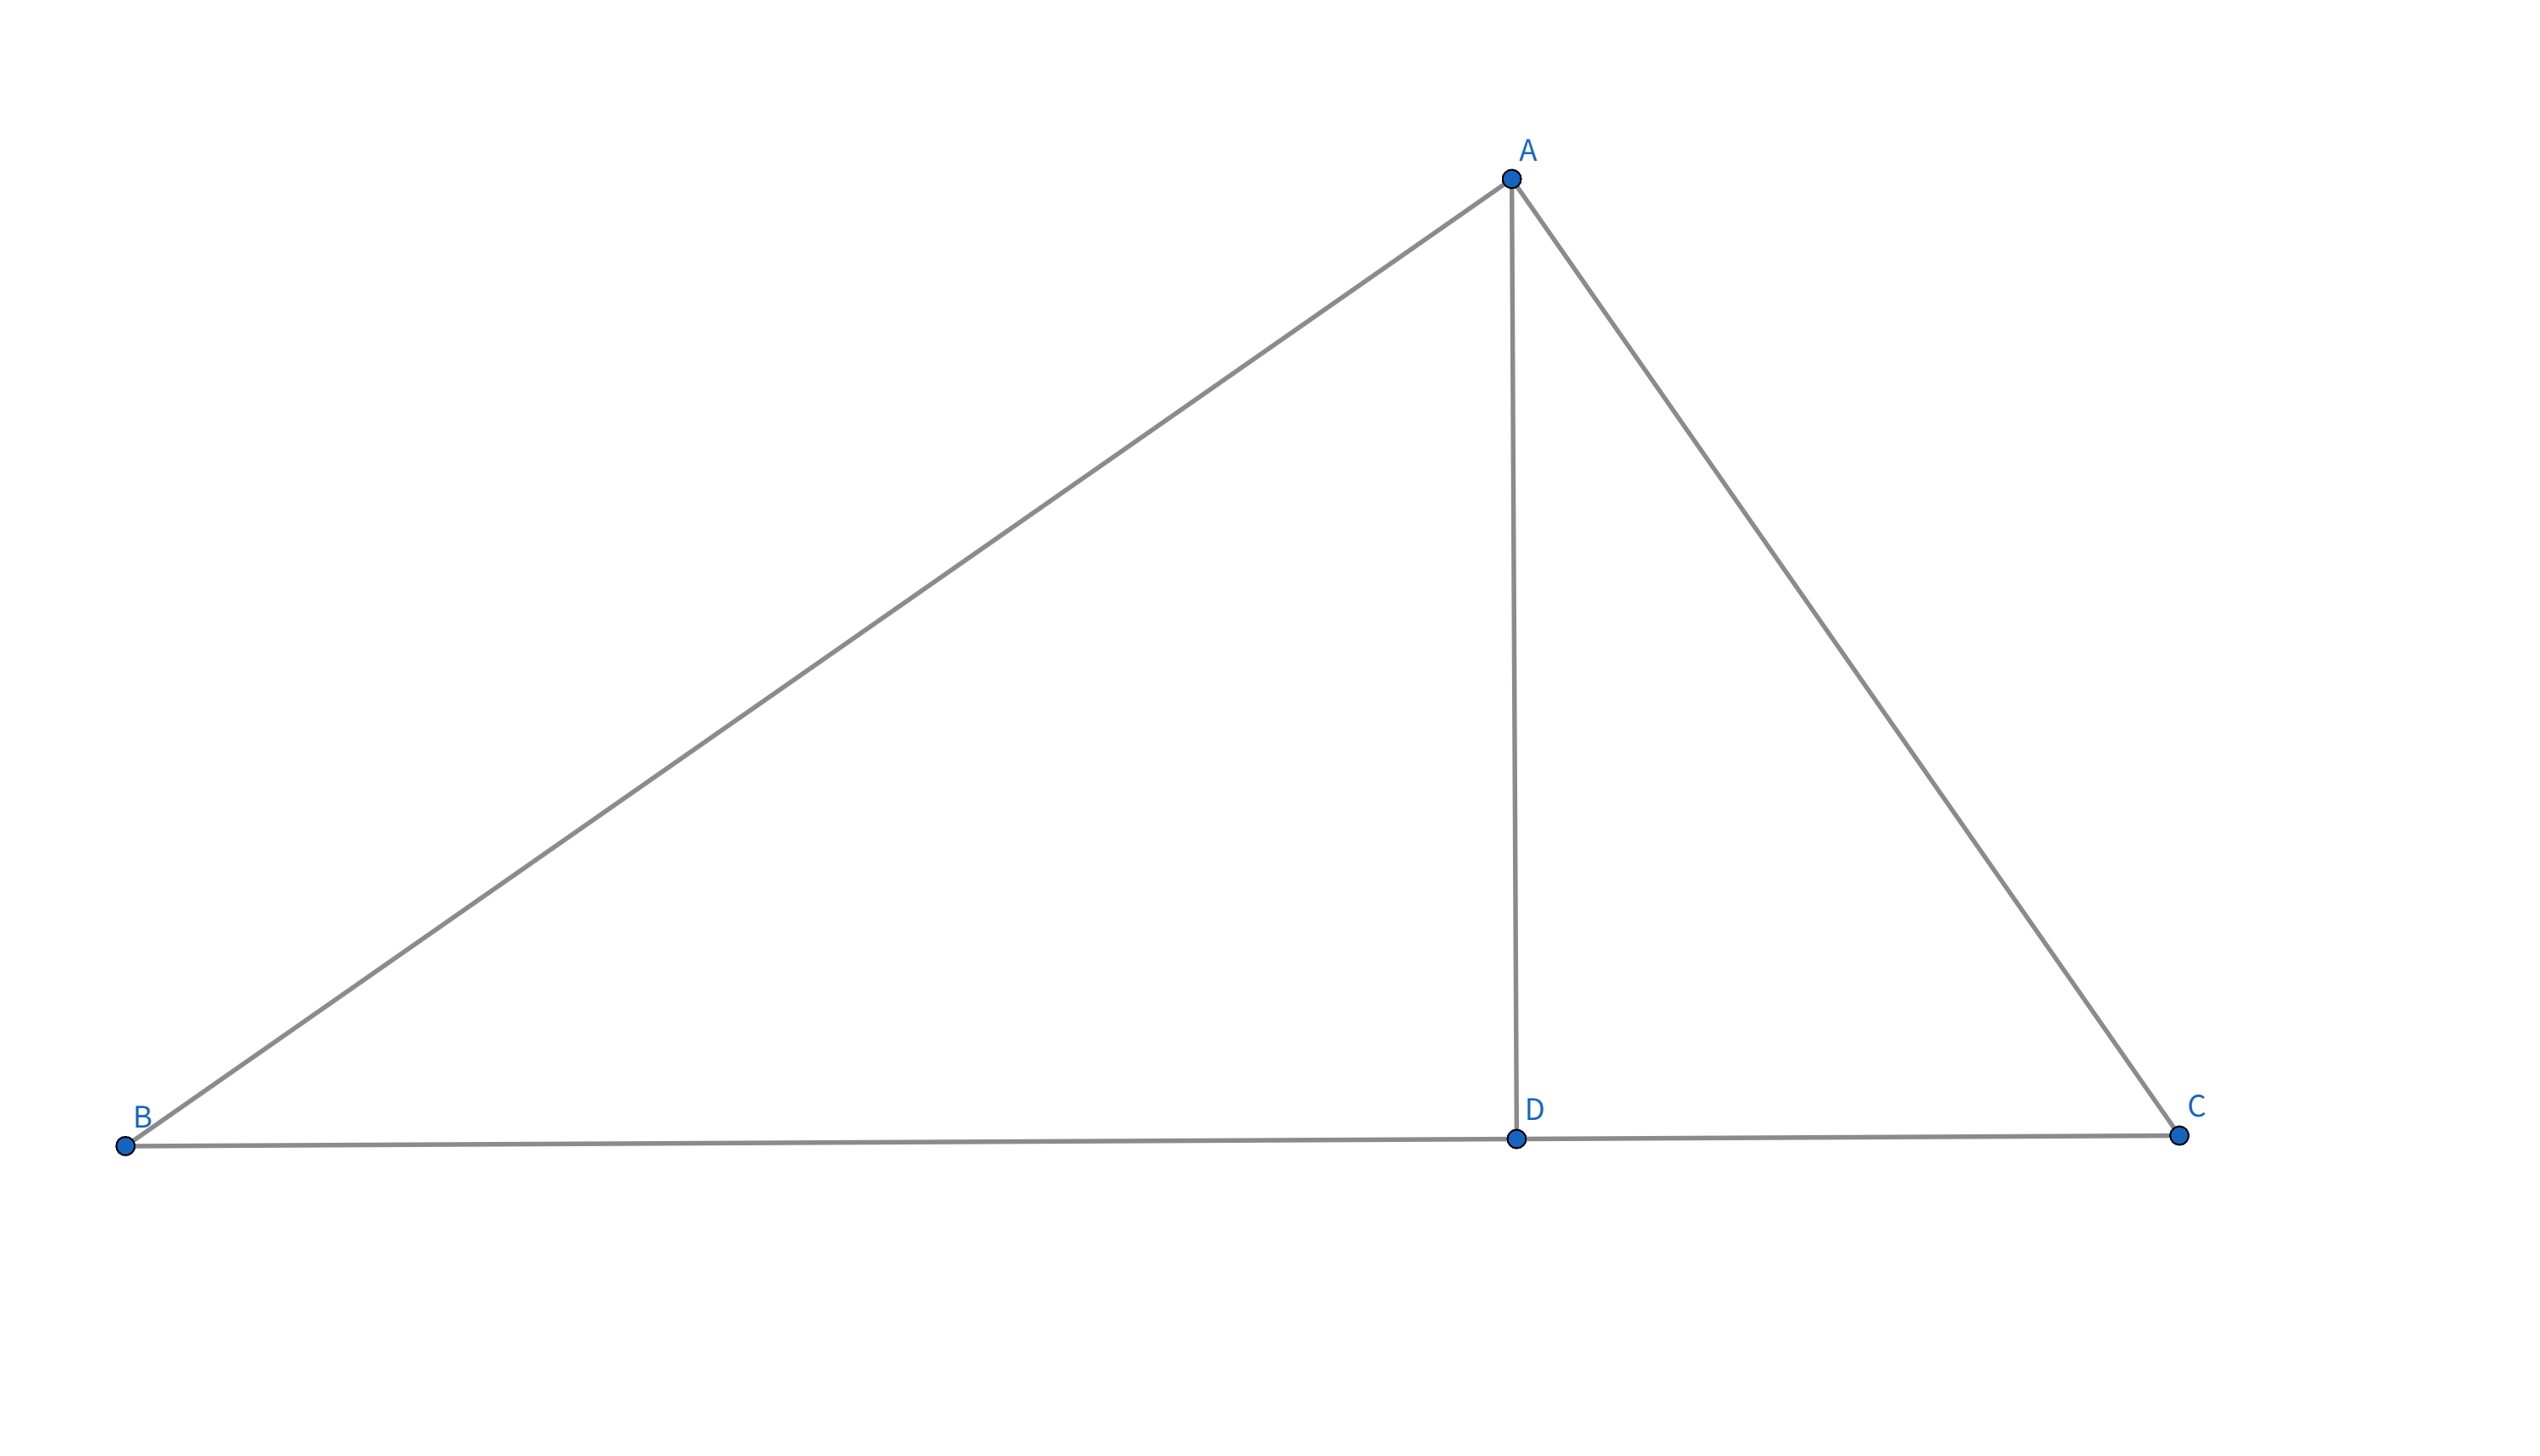
\includegraphics[width=0.8\linewidth]{figures/射影定理.png}
    \caption{射影定理}
    % \label{fig:enter-label}
\end{figure}
